\documentclass[mathserif,t]{beamer}
\usepackage{pgfplots}
\usetikzlibrary{positioning}
\usetikzlibrary{fit}
\usetikzlibrary{backgrounds}
\usetikzlibrary{calc}
\usetikzlibrary{shapes}
\usetikzlibrary{mindmap}
\usetikzlibrary{decorations.text}
\pgfplotsset{compat=1.7}
\usetheme{Boadilla}
\usecolortheme{seagull}
\newcommand{\tikzmark}[1]{\tikz[overlay,remember picture] \node (#1) {};}
\setbeamertemplate{enumerate items}{(\arabic{enumi})}
\setbeamertemplate{itemize items}[circle]
\setbeamercovered{transparent=15}

\newcounter{savedenum}
\newcommand*{\saveenum}{\setcounter{savedenum}{\theenumi}}
\newcommand*{\resume}{\setcounter{enumi}{\thesavedenum}}
\newcommand{\blind}{0}

\usepackage{amsmath,amsthm,amssymb,amsfonts}
\usepackage{enumerate}
\usepackage{graphicx} % Allows including images
\usepackage{color,colortbl}

\usepackage{booktabs} % Allows the use of \toprule, \midrule and \bottomrule in tables
\usepackage{caption}
\usepackage{algorithm} 
\usepackage{algpseudocode}
\usepackage{bbm}
\setbeamertemplate{bibliography item}{}
\setbeamertemplate{theorems}[numbered]
\newtheorem{thm}{Theorem}
\newtheorem{lem}[thm]{Lemma}
\newtheorem{cor}{Corollary}
\newtheorem*{defi*}{Definition}
\newcommand{\G}{c}
\providecommand{\mb}[1]{\boldsymbol{#1}}
\providecommand{\sct}[1]{{\normalfont\textsc{#1}}}
\providecommand{\mt}[1]{\widetilde{#1}}
\newcommand{\Real}{\mathbb{R}}
\newcommand{\Mgc}{MGC}
\newcommand{\mbx}{X}
\newcommand{\mby}{Y}
\newcommand{\GG}{c}
\newcommand{\E}{\hat{E}}

\definecolor{UniBlue}{RGB}{0,26,56}
\definecolor{UniOrange}{RGB}{253,185,19}
\definecolor{UniTitle}{RGB}{192,192,192}
\definecolor{UniText}{RGB}{200,200,200}
\definecolor{OutCirc}{RGB}{185,224,247}
\setbeamerfont{title}{size=\LARGE}
\setbeamerfont{section title}{size=\Huge}
\setbeamercolor{title}{fg=UniTitle}
\setbeamertemplate{frametitle}{\fontfamily{qtm}\LARGE\color{UniOrange}\bfseries\insertframetitle\vskip-6pt\par\hrulefill}
\setbeamercolor{background canvas}{bg=UniBlue}
\setbeamercolor{normal text}{fg=UniText}
\setbeamercolor{structure}{fg=UniText}
\setbeamercovered{invisible}
\setbeamercolor{navigation symbols}{fg=UniOrange, bg=UniOrange}
\setbeamercolor{palette sidebar secondary}{fg=UniOrange,bg=UniOrange}
\setbeamercolor{section in sidebar shaded}{fg=UniOrange,bg=UniOrange}
\setbeamercolor{footlinecolor}{fg=UniOrange,bg=UniOrange}
\setbeamertemplate{navigation symbols}{}
\setbeamertemplate{footline}
{
  \leavevmode%
  \hbox{%
	\hfill
	\hskip5pt%
	\color{UniOrange}
	\insertshortauthor
	\hskip245pt%
	\usebeamercolor[fg]{navigation symbols}%\insertslidenavigationsymbol%
  \insertframenavigationsymbol%
  %\insertsubsectionnavigationsymbol%
  \insertsectionnavigationsymbol%
  %\insertdocnavigationsymbol%
	\hskip15pt%
	\insertshorttitle: \ \insertframenumber/\inserttotalframenumber}
}
\setbeamertemplate{section page}
{
    \begingroup
    \begin{beamercolorbox}[sep=100pt,center]{section title}
        \usebeamerfont{section title}\insertsection\par
    \end{beamercolorbox}
    \endgroup
}

\title[MGC]{\fontfamily{qtm} \bfseries Dependency Discovery via\\
Multiscale Graph Correlation} 
\bigskip
\bigskip
\author[C. Shen]{\large\textcolor{UniTitle}{\textit{Cencheng Shen}}} % Your name
\institute[JHU]{\footnotesize\color{UniTitle}\textit{University of Delaware}\\ % Your institution as it will appear on the bottom of every slide, may be shorthand to save space
\bigskip
\bigskip
\bigskip
\bigskip
\textit{Collaborators: Carey E. Priebe, Joshua T. Vogelstein, Shangsi Wang, Ronak Mehta, Eric Bridgeford, Sambit Panda, Junhao Xiong, Youjin Lee, Qing Wang, Alex Badea, Xu Ting, Mauro Maggioni.\\
\medskip
Acknowledgment: NSF DMS, DARPA SIMPLEX.\\
\medskip
\medskip}}
\date{\footnotesize\color{UniTitle}\footnotesize\textit{}} % Date, can be changed to a custom date
\tikzset{
   invisible/.style={opacity=0},
   visible on/.style={alt=#1{}{invisible}},
   alt/.code args={<#1>#2#3}{%
      \alt<#1>{\pgfkeysalso{#2}}{\pgfkeysalso{#3}} % \pgfkeysalso doesn't change the path
   },
}

\AtBeginSection{\frame{\sectionpage}}

\begin{document}
\bibliographystyle{ieeetr}
\begin{frame}
\titlepage % Print the title page as the first slide
\end{frame}
%1. Intro; 2. it is linear regression and classification; 3. its origin, and why we start investigation; 4. explain title

\setbeamertemplate{section in toc}{\inserttocsectionnumber.~\inserttocsection}
\begin{frame}
\frametitle{Overview} % Table of contents slide, comment this block out to remove it
\tableofcontents % Throughout your presentation, if you choose to use \section{} and \subsection{} commands, these will automatically be printed on this slide as an overview of your presentation
\end{frame}

\section{Motivation}
\begin{frame}{Motivation}
Given paired data $(\mathcal{X}_{n},\mathcal{Y}_{n})=\{(x_{i},y_{i}) \in \Real^{p} \times \Real^{q}, \ \mbox{ for } i=1,\ldots,n\}$,
\pause
\begin{itemize}[<+->]
\item Are they related?
\item How are they related?
\end{itemize}
\pause
\medskip
%If the data has no dependency signal, it is futile to build a joint model or to predict one data from another. 

\begin{table}
\centering
\begin{tabular}{|c|c|}
\hline
\textbf{$X$} & \textbf{$Y$}   \\
\hline
%  Oracle \Mgc  & \textbf{50}  & 60 & \textbf{70} & \textbf{135} \\
% \hline
brain connectivity  & creativity / personality \\
\hline 
brain shape & health \\
\hline
gene / protein & cancer\\
\hline
social networks & attributes \\
\hline
anything & anything else \\
\hline
\end{tabular}
\end{table}
\end{frame}

\begin{frame}{Formal Definition of Independence Testing}
\begin{align*}
& (x_{i},y_{i}) \stackrel{i.i.d.}{\sim} F_{XY}, \ \ i=1, \ldots, n\\
& \\
& H_{0}: F_{XY}=F_{X}F_{Y},\\
& H_{A}: F_{XY} \neq F_{X}F_{Y}.
\end{align*}

\pause
\medskip
A dependence / correlation measure is any statistic that can be used to test the above hypothesis.

\pause
\medskip
We desire a universally consistent test via some dependence measure, i.e., the testing power converges to $1$ as $n \rightarrow \infty$ against any dependent $F_{XY}$.

\pause
\medskip
Without loss of generality, we shall assume $F_{XY}$ has finite second moments.

%\pause
%\medskip
%For a given test statistic (MGC, Dcorr, HHG, HSIC, etc.), finite-sample testing is almost always carried out via a permutation test (unless the null distribution is known, which is generally not the case), and the null is rejected when the p-value is sufficiently small.

%\pause
%\medskip
%For any scientist trying to identify some relationship from their data, they desire a test statistic of high finite-sample testing power (rather than asymptotically)!
%The power of a test is defined as the probability that it correctly rejects the null when the null is indeed false, and has power equal to the type $1$ error level when the null is true. And a test is universally consistent if its power converges to $1$ as $n \rightarrow \infty$ whenever $f_{xy} \neq f_x f_y$.
\end{frame}

\begin{frame}{Benchmarks}
   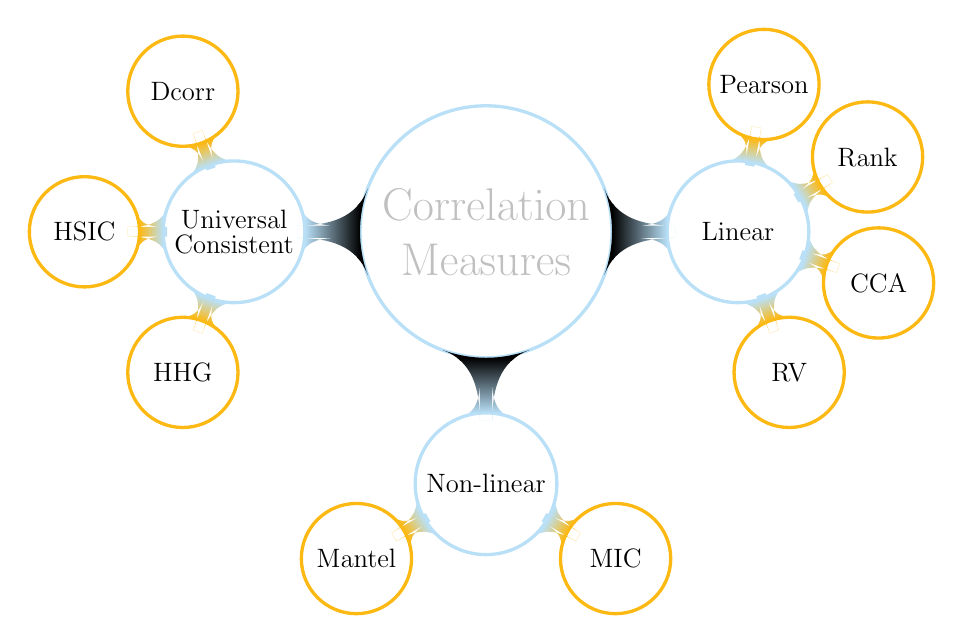
\begin{tikzpicture}[mindmap,
         concept/.append style={fill={none}},
         root concept/.style={concept color=OutCirc},
         level 1 concept/.append style=
         {every child/.style={concept color=OutCirc},level distance = 32mm},
         level 2 concept/.append style=
         {every child/.style={concept color=UniOrange},level distance = 19mm},
         every node/.append style={align=center,scale=0.8},
      ]
      \node [concept,font=\huge,color=OutCirc] {\textcolor{UniTitle}{Correlation Measures}}
      child[grow=0, visible on=<3->] {node[concept] {\large Linear}
         child[grow=80, visible on=<3->]{node[concept] {\large Pearson}}
         child[grow=30, visible on=<3->]{node[concept] {\large Rank}}
         child[grow=-20, visible on=<3->]{node[concept] {\large CCA}}
         child[grow=-70, visible on=<3->]{node[concept] {\large RV}}
      }
      child[grow=-90,visible on=<4->] {node[concept] {\large Non-linear}
         child[grow=-30,visible on=<4->]{node[concept] {\large MIC}}
        % child[grow=270,visible on=<3->]{node[concept] {\large HHG}}
				child[grow=210,visible on=<4->]{node[concept] {\large Mantel}}
      }
      child[grow=180,visible on=<5->] {node[concept] {\large Universal \\ Consistent}
         child[grow=110,visible on=<5-> ] {node[concept] {\large Dcorr}}
         child[grow=180,visible on=<5->] {node[concept] {\large HSIC}}
         child[grow=250,visible on=<5->] {node[concept] {\large HHG}}
      };
      %\node at (0,0) [inner sep=9mm,decorate,circle,decoration=
      %{text along path,text={}}] {};
      %\draw decorate[decoration={text along path,text={Equally Effective}}]
      %{(-3,0) arc (135:45:.5cm)};

   \end{tikzpicture}
\end{frame}

\begin{frame}{Motivations}
Modern data sets may be \textbf{high-dimensional, nonlinear, noisy, of limited sample size, structured, from disparate spaces}. Thus we desire a test that

\pause
\medskip
\begin{itemize}[<+->]
\item is consistent against all dependencies;
\item has good finite-sample testing performance;
\item is easy to understand and efficient to implement;
\item *provides insights into the dependency structure.
\end{itemize}
\pause
\medskip
%Existing method has pros and cons with respect to each point. \\
%
%\pause
%\medskip
To that end, we propose the \textbf{multiscale graph correlation} in [\textit{Shen et al.(2018)}].
\end{frame}


\section{Methodology}
\begin{frame}{Flowchart of \Mgc}

   \makebox[\textwidth][c]{%
      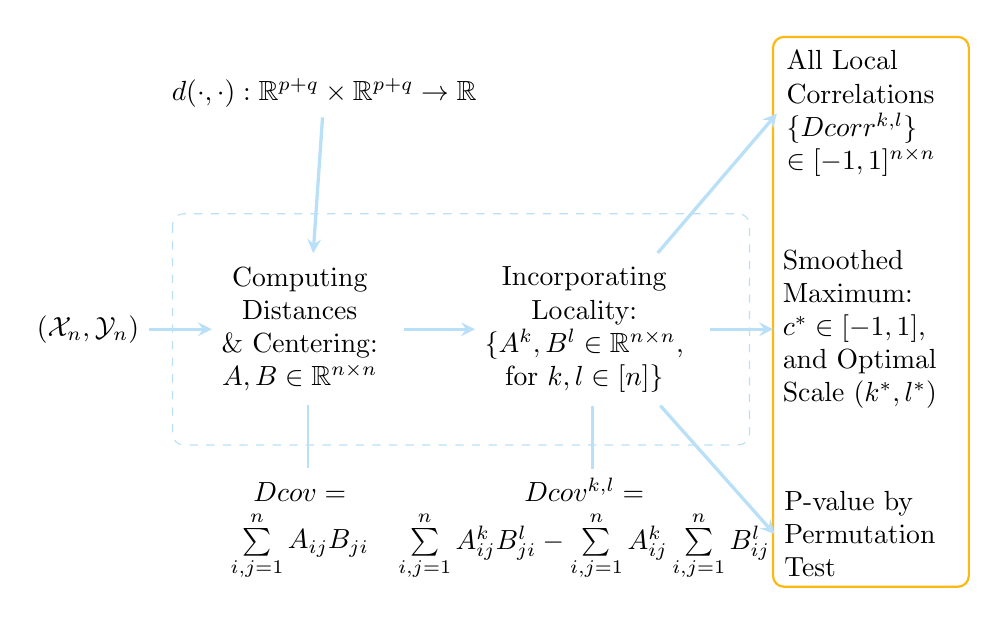
\begin{tikzpicture}[
            outpt/.style={->,OutCirc,very thick},
						outpt2/.style={-,OutCirc,thick},
            >=stealth,
         every node/.append style={align=left}]
				\node (source) at (0,0){$(\mathcal{X}_{n},\mathcal{Y}_{n})$};
				\node (source2)at (3,3){$d(\cdot,\cdot): \mathbb{R}^{p+q} \times \mathbb{R}^{p+q} \rightarrow \mathbb{R}$};
				\pause
         \node (kaela)[right=0.8cm of source]{\begin{tabular}{@{}c}Computing \\ Distances \\ \& Centering: \\ $A, B \in \mathbb{R}^{n \times n}$\end{tabular}};
				\draw[outpt](source)--(kaela);
				\draw[outpt](source2)--(kaela);
				\pause
				\node (dc)[below=0.8cm of kaela]{\begin{tabular}{@{}c} $Dcov =$ \\ $\sum\limits_{i,j=1}^{n} A_{ij}B_{ji}$ \end{tabular}};
				\draw[outpt2](kaela)--(dc);
				\pause          
            \node (accessfile) [right=0.9cm of kaela] {\begin{tabular}{@{}c}Incorporating \\ Locality: \\ $\{A^{k}, B^{l} \in \mathbb{R}^{n \times n}$, \\ for $k,l \in [n]\}$ \end{tabular}};
            \draw[outpt](kaela)--(accessfile);
						\pause
						\node (dc2)[below=0.8cm of accessfile]{\begin{tabular}{@{}c} $Dcov^{k,l} =$ \\ $\sum\limits_{i,j=1}^{n} A_{ij}^{k}B_{ji}^{l}-\sum\limits_{i,j=1}^{n} A_{ij}^{k} \sum\limits_{i,j=1}^{n} B_{ij}^{l}$ \end{tabular}};
				\draw[outpt2](accessfile)--(dc2);
            % Draw background
            \begin{pgfonlayer}{background}
               % Left-top corner of the background rectangle
               \path (kaela.west |- kaela.north)+(-0.5,0.5) node (a) {};
               % Right-bottom corner of the background rectanle
               \path (accessfile.east |- accessfile.south)+(+0.5,-0.5) node (c) {};
               % Draw the background
               \path[rounded corners, draw=OutCirc, dashed]
               (a) rectangle (c);
            \end{pgfonlayer}
         \pause
            \node (screen)[above right=1.2cm of accessfile]{All Local \\ Correlations \\ $\{Dcorr^{k,l}\}$\\$\in [-1,1]^{n \times n}$};
						\draw[outpt](accessfile)--(screen.west);
						\pause   
            \node (braille)[right =0.8cm of accessfile]{Smoothed \\ Maximum: \\ $c^{*} \in [-1,1]$, \\and Optimal \\ Scale $(k^*,l^*)$};
						\draw[outpt](accessfile)--(braille);
						\pause   
            \node (enlarge)[below =0.8cm of braille]{P-value by \\ Permutation \\ Test};
						\draw[outpt](accessfile)--(enlarge.west);
            \begin{pgfonlayer}{background}
               % Left-top corner of the background rectangle
               \path (screen.west |- screen.north)+(-0.05,0.05) node (a) {};
               % Right-bottom corner of the background rectanle
               \path (enlarge.east |- enlarge.south)+(0.3,0) node (c) {};
               % Draw the background
               \path[rounded corners, draw=UniOrange,thick]
               (a) rectangle (c);
            \end{pgfonlayer}
      \end{tikzpicture}
   }
\end{frame}

\begin{frame}{Computing Distance and Centering}
\textbf{Input:} $\mathcal{X}_{n}=[x_{1},\ldots,x_{n}]$ as the data matrix with each column representing one sample observation, and similarly $\mathcal{Y}_{n}$. A distance or kernel function $d(\cdot,\cdot): \mathbb{R}^{p+q} \times \mathbb{R}^{p+q} \rightarrow \mathbb{R}$, by default the Euclidean distance.\\
\pause
\medskip
\textbf{Distance Computation: } Let $\tilde{A}$ be the $n \times n$ Euclidean distance matrices of $\mathcal{X}_{n}$:
\begin{align*}
\tilde{A}_{ij}=d(x_i,x_j)=\|x_{i}-x_{j}\|_{2},
\end{align*}
and similarly $\tilde{B}$ from $\mathcal{Y}_{n}$.\\

\pause
\medskip
\textbf{Centering:} Then we center $\tilde{A}$ and $\tilde{B}$ by columns, with the diagonals excluded:
\begin{equation}
\label{localCoef2}
    A_{ij}=
    \begin{cases}
      \tilde{A}_{ij}-\frac{1}{n-1}\sum_{s=1}^{n} \tilde{A}_{sj}, & \text{if $i \neq j$}, \\    
     0, & \text{if $i=j$};
    \end{cases}
\end{equation}
similarly for $B$. 
\end{frame}

%\begin{frame}{Examples}
%A few examples of $\G$:
%\begin{itemize}[<+->]
%\item The Pearson's product-moment correlation coefficient by taking $a_{ij}=x_i$ and $b_{ij}=y_i$.
%\item The Spearman and Kendall's rank correlations by setting $a_{ij}$ to be $rank(x_i)-rank(x_j)$ and $sign(x_i-x_j)$ respectively.
%\item The Mantel coefficient [\textit{Mantel (1967)}]\cite{Mantel1967} by using $a_{ij}=|x_i-x_j|_{2}$ (i.e. Euclidean distance).
%\item The distance correlation [\textit{Szekely et al.(2007)}]\cite{SzekelyRizzoBakirov2007} by using the doubly-centered distance entries for $a_{ij}$ and $b_{ij}$.
%\item The modified distance correlation [\textit{Szekely and Rizzo (2013)}] \cite{SzekelyRizzo2013a} by slightly tweaking $a_{ij}/b_{ij}$ of dcorr.
%\end{itemize}
%\end{frame}

\begin{frame}{Incorporating the Locality Principle}
\pause
\textbf{Ranking:} Define $\{R^{A}_{ij}\}$ as the ``rank'' of $x_i$ relative to $x_j$, that is, $R^{A}_{ij}=k$ if $x_i$ is the $k^{th}$ closest point (or ``neighbor'') to $x_j$, as determined by ranking the set $\{\tilde{A}_{1j},\tilde{A}_{2j},\ldots,\tilde{A}_{nj}\}$ by ascending order. Similarly define $R^{B}_{ij}$ for the $y$'s. 

\pause
\medskip
For any $(k,l) \in [n]^2$, define the rank truncated matrices $A^{k}, B^{l}$, and the joint distance matrix $C^{kl}$ as
\begin{align*}
A_{ij}^{k} &=A_{ij} \mb{I}(R^{A}_{ij} \leq k), \\
B_{ij}^{l} &=B_{ij} \mb{I}(R^{B}_{ij} \leq l). 
\end{align*}

\pause
\medskip
When ties occur, minimal rank is recommended, e.g., if $\mby$ only takes two value, $R^{B}_{ij}$ takes value in $\{1,2\}$ only. We assume no ties for each of presentation.
\end{frame}

\begin{frame}{Local Distance Correlations}
\pause
\textbf{A Family of Local Correlations:} 
Let $\circ$ denote the entry-wise product, $\E(\cdot)=\frac{1}{n(n-1)}\sum_{i \neq j}^{n} (\cdot)$ denote the diagonal-excluded sample mean of a square matrix, then the sample local covariance, variance, and correlation are defined as:
\pause
\begin{align*}
dCov^{k,l}(\mathcal{X}_{n},\mathcal{Y}_{n}) &= \E(A^{k} \circ B^{l'})- \E(A^{k})\E(B^{l}),\\
dVar^{k}(\mathcal{X}_{n}) &=\E(A^{k} \circ A^{k'})- \E^2(A^{k}), \\
dVar^{l}(\mathcal{Y}_{n}) &=\E(B^{l} \circ B^{l'})- \E^2(B^{l}), \\
dCorr^{k,l}(\mathcal{X}_{n},\mathcal{Y}_{n}) &=dCov^{k,l}(\mathcal{X}_{n},\mathcal{Y}_{n}) / \sqrt{dVar^{k}(\mathcal{X}_{n}) \cdot dVar^{l}(\mathcal{Y}_{n})}.
\end{align*}
\pause
for $k,l=1,\ldots,n$. If $dVar^{k}(\mathcal{X}_{n}) \cdot dVar^{l}(\mathcal{X}_{n}) \leq 0$, we set $dCorr^{kl}(\mathcal{X}_{n},\mathcal{Y}_{n})=0$ instead. 

\pause
\medskip
There are a maximum of $n^2$ different local correlations. At $k=l=n$, $dCorr^{kl}(\mathcal{X}_{n},\mathcal{Y}_{n})$ equals the ``global'' distance correlation $dCorr(\mathcal{X}_{n},\mathcal{Y}_{n})$ by \textit{Szekely et al.(2007)}.
\end{frame}

%\begin{frame}{MGC}
%\pause
%\textbf{MGC as optimal local correlation:} In $\{dCorr^{kl}(X_{n},Y_{n})\}$, we shall take the ``optimal'' local correlation as the \Mgc~statistic $\G^{*}(X_{n},Y_{n})$. 

%\pause
%\medskip
%However, directly taking the maximum local correlation $\max_{(k,l) \in [n]^2}\{dCorr^{k,l}(X_{n},Y_{n})\}$ will yield a biased statistic under independence, i.e., the maximum is always larger than $0$ in expectation even under independent relationship.

%\pause
%\medskip
%Instead, we take a smoothed maximum by:
%\begin{itemize}[<+->]
%\item Pick a threshold $\tau \geq 0$;
%\item Compute the largest connected component $R=\{(k,l)$ such that $dCorr^{kl}(X_{n},Y_{n})>\max\{\tau, dCorr^{nn}(X_{n},Y_{n})\} \}$;
%\item Within the significant region $R$, set $\GG^{*}(X_{n},Y_{n})=\max_{ (k,l) \in R} \{dCorr^{k,l}(X_{n},Y_{n})\}$;
%\item If the number of elements in $R$ is less than $2n$, or the $\GG^{*}(X_{n},Y_{n})$~is no more than $dCorr^{nn}(X_{n},Y_{n})$, take $\GG^{*}(X_{n},Y_{n})=dCorr^{nn}(X_{n},Y_{n})$ instead.
%\end{itemize}
%\end{frame}

\begin{frame}{Smoothed Maximum $c^{*}(\mathcal{X}_{n},\mathcal{Y}_{n})$}
One would like to use the optimal local correlation for testing.\\
\pause
\medskip

But directly taking the maximum local correlation 
\begin{align*}
\max_{(k,l) \in [n]^2}\{Dcorr^{k,l}(\mathcal{X}_{n},\mathcal{Y}_{n})\}
\end{align*}
will yield a biased statistic under independence, i.e., the maximum is always larger than $0$ in expectation even under independent relationship!

\pause
\medskip
Instead, we take a smoothed maximum, by finding a connected region in the local correlation map with significant local correlatons -- if such a region exists, use the maximum within the region.
\end{frame}

\begin{frame}{Smoothed Maximum}
Pick a threshold $\tau \geq 0$ (we choose by an approximate null distribution of $Dcorr$, which is symmetric beta and converges to $0$ as $n \rightarrow \infty$), compute the set
\begin{align*}
\{(k,l) \mbox{ such that } Dcorr^{k,l}(\mathcal{X}_{n},\mathcal{Y}_{n})>\max\{\tau, Dcorr(\mathcal{X}_{n},\mathcal{Y}_{n})\} \},
\end{align*}
\pause
and calculate the largest connected component $R$ of the set.

\pause
\medskip
If there are sufficiently many elements in $R$ $(>2n)$, take the maximum correlation within $R$ as \Mgc~statistic $c^{*}(\mathcal{X}_{n},\mathcal{Y}_{n})$, 
\pause
and set the neighborhood pair as the optimal scale $(k^*,l^*)$.
%\pause
%\medskip
%$\tau$ has negligible effect on theoretical properties of \Mgc~but is somewhat important for limited-sample performance. More details on smoothing can be found in [\textit{Shen et al.(2018)}].
\end{frame}

\begin{frame}{Permutation Test}
To get a p-value by \Mgc~for any given data, we utilize the permutation test: randomly permute index of the second data set for $r$ times, compute the permuted \Mgc~statistic $c^{*}(\mathcal{X}_{n},\mathcal{Y}_{n}^{\pi})$ for each permutation $\pi$, and estimate 
\begin{align*}
Prob(c^{*}(\mathcal{X}_{n},\mathcal{Y}_{n})>c^{*}(\mathcal{X}_{n},\mathcal{Y}_{n}^{\pi}))
\end{align*}
as the p-value.
\pause
\medskip

This is a standard nonparametric testing procedure employed by Mantel, Dcorr, HHG, HSIC, where the null distribution of the dependency measure cannot be exactly derived.
\end{frame}

\begin{frame}{Computation Complexity}
\begin{itemize}
\item Distance computation takes $\mathcal{O}(n^2 \max(p,q))$
\item Centering takes $\mathcal{O}(n^2)$
\item Ranking takes $\mathcal{O}(n^2 log(n))$
\item \textbf{All local correlations can be iteratively computed in $\mathcal{O}(n^2)$}
\item The smoothed maximum takes $\mathcal{O}(n^2)$
\item Storage requirement is $\mathcal{O}(n^2)$
\end{itemize}

\pause
Overall, \Mgc~can be computed in $\mathcal{O}(n^2 \max(p,q,\log n))$. Without the ranking process, the global correlation (Dcorr) waives the $\log n$ part and takes $\mathcal{O}(n^2 \max(p,q))$.

\pause
\medskip
The permutation test takes $\mathcal{O}(n^2 \max(r,p,q,\log n))$ for $r$ random permutations.
\pause
\medskip

On a standard PC with Matlab, testing $n=1000$ takes about $1$ minutes.
\end{frame}

\begin{frame}{Examples}
\pause
   \makebox[\textwidth][c]{%
      \begin{tikzpicture}[
            outpt/.style={->,OutCirc,very thick},
            >=stealth,
         every node/.append style={align=left}]
			\node (source) at (0,0)[]{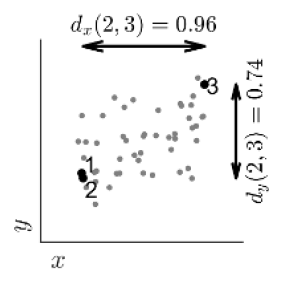
\includegraphics[width=.22\textwidth]{linear.png}};
			\pause
\node (kaela)[right=of source]
    {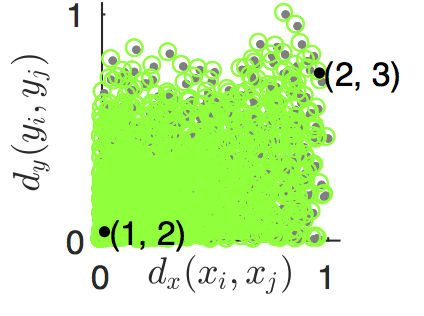
\includegraphics[width=.28\textwidth]{Fig1B.png}};
\draw[outpt](source)--(kaela);
\pause
\node (result)[right=of kaela] {$Dcorr(\mathcal{X}_{n},\mathcal{Y}_{n}) =0.15$ \\ $MGC(\mathcal{X}_{n},\mathcal{Y}_{n})=0.15$ \\ p-vals: $<0.001$};
\draw[outpt](kaela)--(result);
	
	\pause

			\node (source2)[below=of source]{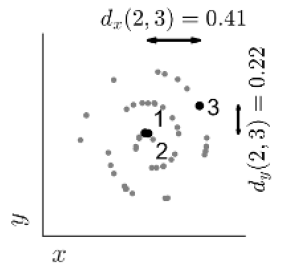
\includegraphics[width=.22\textwidth]{spiral.png}};
			\pause
\node (kaela2)[right=of source2]
    {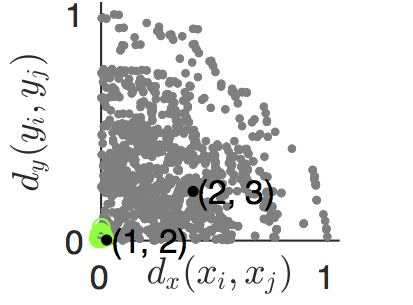
\includegraphics[width=.28\textwidth]{Fig8B.png}};
\draw[outpt](source2)--(kaela2);
\pause
\node (result2)[right=of kaela2] {$Dcorr(\mathcal{X}_{n},\mathcal{Y}_{n}) =0.01$ \\ $MGC(\mathcal{X}_{n},\mathcal{Y}_{n})=0.13$ \\ p-vals: $0.3$ vs $<0.001$};
\draw[outpt](kaela2)--(result2);
\end{tikzpicture}
   }
\end{frame}

\begin{frame}{\Mgc~is applicable to similarity / kernel matrix}
%1. $MGC= Mantel=Dcorr=1$ against linear relationships; \\
%\ \ \ \ \ \ \ \ \ \ \ \ \ \ \ \ \ \ \ \ \ \ \ \ \ \ \ \ \ \ \ \ \ \ \ \ \ \ \ $=0$ against independence.\\
%\pause
\begin{thm}[Transforming kernel to distance]
Given any kernel function $k(\cdot,\cdot)$, define an induced semi-metric as 
\begin{center}
$d(i,j)=1-k(i,j) / \max_{i,j=1,\ldots,n}\{k(i,j)\}$.
\end{center}
%Then $d(\cdot,\cdot)$ is of strong negative type, and the resulting MGC is universally consistent.
\end{thm}
\pause
\medskip
Namely, given a sample kernel matrices $K_{n \times n}$, one can compute the induced distance matrix by 
\begin{center}
$D=J-K/\max_{i,j \in [1,\ldots,n]^2}\{K(i,j)\}$,
\end{center}
and apply MGC or other distance-based correlation to the induced distance matrices.\\
\pause
\medskip
The kernel correlation HSIC is equivalent to distance correlation. 
\end{frame}
%\begin{frame}{Advantages of \Mgc}
%3. *The local correlations provide an encoding of the dependency structure. 

%\pause
%\bigskip

%4. Efficient implementation in $\mathcal{O}(n^2 log n)$.

%\pause
%\bigskip

%MGC shares the same intrinsic idea as in nonlinear embedding, random forest, deep learning.
%\end{frame}

\section{Theoretical Properties}
\begin{frame}{Basic Properties of Sample \Mgc}
\begin{thm}[Well-behaved Correlation Measure]
\pause
1. Boundedness: $c^{*}(\mathcal{X}_{n},\mathcal{Y}_{n}) \in [-1,1]$.\\
\pause
\medskip
2. Symmetric: $c^{*}(\mathcal{X}_{n},\mathcal{Y}_{n}) =c^{*}(\mathcal{Y}_{n},\mathcal{X}_{n})$.\\
\pause
\medskip
3. Invariant: $c^{*}(\mathcal{X}_{n},\mathcal{Y}_{n})$ is invariant to any distance-preserving transformations $\phi,\delta$ applied to $\mathcal{X}_{n}$ and $\mathcal{Y}_{n}$ each (i.e., rotation, scaling, translation, reflection).\\
\pause
\medskip
4. 1-Linear: $c^{*}(\mathcal{X}_{n},\mathcal{Y}_{n})=1$ if and only if $F_{X}$ is non-degenerate and $(X, u Y)$ are dependent via an isometry for some non-zero constant $u$.\\
\end{thm}
\end{frame}

\begin{frame}{Consistency of Sample \Mgc}
\begin{thm}[Consistency]
\pause
1. 0-Indep: $c^{*}(\mathcal{X}_{n},\mathcal{Y}_{n}) \stackrel{n \rightarrow \infty}{\rightarrow}0$ if and only if independence.\\
\pause
\medskip
2. Valid Test: Under the permutation test, Sample \Mgc~is a valid test, i.e., it controls the type 1 error level $\alpha$.\\
\pause
\medskip
3. Consistency: At any type 1 error level $\alpha$, testing power $\beta(c^{*}(\mathcal{X}_{n},\mathcal{Y}_{n})) \stackrel{n \rightarrow \infty}{\rightarrow} 1$ against any dependent $F_{\mbx \mby}$.\\
\end{thm}
\pause
\medskip
The distance correlation also shares the same properties.
\end{frame}

\begin{frame}{Defining Population \Mgc}
%\begin{defi*}
Suppose $(\mbx,\mby), (\mbx',\mby'), (\mbx'',\mby''), (\mbx''',\mby''')$ are \emph{iid} as $F_{XY}$. 
\pause
Let $\mb{I}(\cdot)$ be the indicator function, define two random variables
\begin{align*}
\mb{I}_{\mbx,\mbx'}^{\rho_{k}} &=\mb{I}(\int_{B(\mbx,d(\mbx',\mbx))} dF_\mbx(u) \leq \rho_k)  \\
\mb{I}_{\mby',\mby}^{\rho_{l}} &=\mb{I}(\int_{B(\mby',d(\mby'-\mby))} dF_\mby(u) \leq \rho_l)
\end{align*}
for $\rho_{k},\rho_{l} \in [0,1]$.
\pause
Further define
\begin{align*}
g^{\rho_{k}}_{\mbx} &=(d(\mbx,\mbx') - d(\mbx,\mbx'')) \mb{I}_{\mbx,\mbx'}^{\rho_{k}} \\
g^{\rho_{l}}_{\mby'} &=(d(\mby',\mby) - d(\mby',\mby''')) \mb{I}_{\mby',\mby}^{\rho_{l}}
\end{align*}
\pause
The population local covariance can be defined as
\begin{align*}
%\label{eq:dcov2}
Dcov^{\rho_{k}, \rho_{l}}(\mbx,\mby) = E(g^{\rho_{k}}_{\mbx} g^{\rho_{l}}_{\mby'}) - E(g^{\rho_{k}}_{\mbx}) E(g^{\rho_{l}}_{\mby'}).
\end{align*}
\pause
Normalizing and taking a smoothed maximum yield population \Mgc.
%\end{defi*}
\end{frame}

\begin{frame}{Sample to Population}
\pause
Under the Euclidean distance, the population version can be equivalently defined via an integral of characteristic functions of $F_{XY}-F_{X}F_{Y}$ with respect to a non-negative weight function $w(t,s)$.
\pause 
\medskip

For general metric or kernel function $d(\cdot,\cdot)$, the population version can also be defined as the integral of $d(X,X')d(Y,Y')$ with respect to $(F_{XY}-F_{X}F_{Y})(F_{X'Y'}-F_{X'}F_{Y'})$.
\pause
\medskip

When the metric is of strong negative type or the kernel is characteristic, $c^{*}(X,Y)=0$ if and only if independence. For arbitrary metric or kernel, the if direction is still true but not the only if direction.
%Under Euclidean distance, the population version can be equivalently defined via characteristic functions of $F_{XY}$:
%\begin{align*}
%Dcov^{\rho_{k}=1, \rho_{l}=1}(\mbx,\mby) = \int_{t,s} |g_{XY}(t,s)-g_{X}(t)g_{Y}(s)|^2 dw(t,s)
%\end{align*}
%with respect to a non-negative weight function $w(t,s)$ on $(t,s) \in \mathbb{R}^{p} \times \mathbb{R}^{q}$. 
%\pause 
%The weight function is defined as:
%\begin{align*}
%		w(t,s) &=  (d_{p}d_{q} |t|^{1+p}|s|^{1+q})^{-1},
%\end{align*}
%where $d_{p}=\frac{\pi^{(1+p)/2}}{\Gamma((1+p)/2)}$ is a non-negative constant tied to the dimensionality $p$, and $\Gamma(\cdot)$ is the complete Gamma function.\\
%\pause
%\medskip
%Can be similarly adapted to the local correlation.
\end{frame}

\begin{frame}{Theoretical Advantages of \Mgc}
\begin{thm}[Convergence, Mean and Variance]
\pause
1. 0-Indep: When the metric is of strong negative type or the kernel is characteristic, $c^{*}(X,Y) =0$ if and only if independence.\\
\pause
\medskip
2. Convergence: $c^{*}(\mathcal{X}_{n},\mathcal{Y}_{n}) \stackrel{n \rightarrow \infty}{\rightarrow} c^{*}(X,Y)$.\\
\pause
\medskip
3. Almost Unbiased: $E(c^{*}(\mathcal{X}_{n},\mathcal{Y}_{n})) =c^{*}(X,Y)+\mathcal{O}(1/n)$.\\
\pause
\medskip
4. Diminishing Variance: $Var(c^{*}(\mathcal{X}_{n},\mathcal{Y}_{n})) =\mathcal{O}(1/n)$.\\
\end{thm}
\pause
\medskip
The last three properties also hold for any local correlation by $(\rho_{k},\rho_{l})=(\frac{k-1}{n-1},\frac{l-1}{n-1})$, as well as the distance correlation, i.e., $k=l=n$.
%Same boundedness, symmetric, invariant, 1-linear properties as sample version.\\
\end{frame}

\begin{frame}{Theoretical Advantages of \Mgc}
%1. $MGC= Mantel=Dcorr=1$ against linear relationships; \\
%\ \ \ \ \ \ \ \ \ \ \ \ \ \ \ \ \ \ \ \ \ \ \ \ \ \ \ \ \ \ \ \ \ \ \ \ \ \ \ $=0$ against independence.\\
%\pause
\begin{thm}[Advantages of Population \Mgc~vs Dcorr]
\pause
1. For any dependent $F_{XY}$, $c^{*}(X,Y) \geq Dcorr(X,Y)$. \\
\pause
\medskip
2. There exists dependent $F_{XY}$ such that $c^{*}(X,Y)>Dcorr(X,Y)$.\\
\end{thm}
\pause
As \Mgc~and Dcorr share similar variance and same mean under the null, the first moment advantage in the alternative is translated to the testing power. 
\pause
\begin{thm}[Optimal Scale of \Mgc~Implies Geometry Structure]
\pause
If the relationship is linear (or with independent noise), the global scale is always optimal and $c^{*}(X,Y)=Dcorr(X,Y)$.\\
\pause
\medskip
Conversely, the optimal scale being local, i.e., $c^{*}(X,Y)>Dcorr(X,Y)$, implies a non-linear relationship.
\end{thm}
\end{frame}

\section{Simulations and Experiments}
\begin{frame}{Visualizations of $20$ Simulation Settings}
\pause
\begin{figure}[ht]
  \centering
  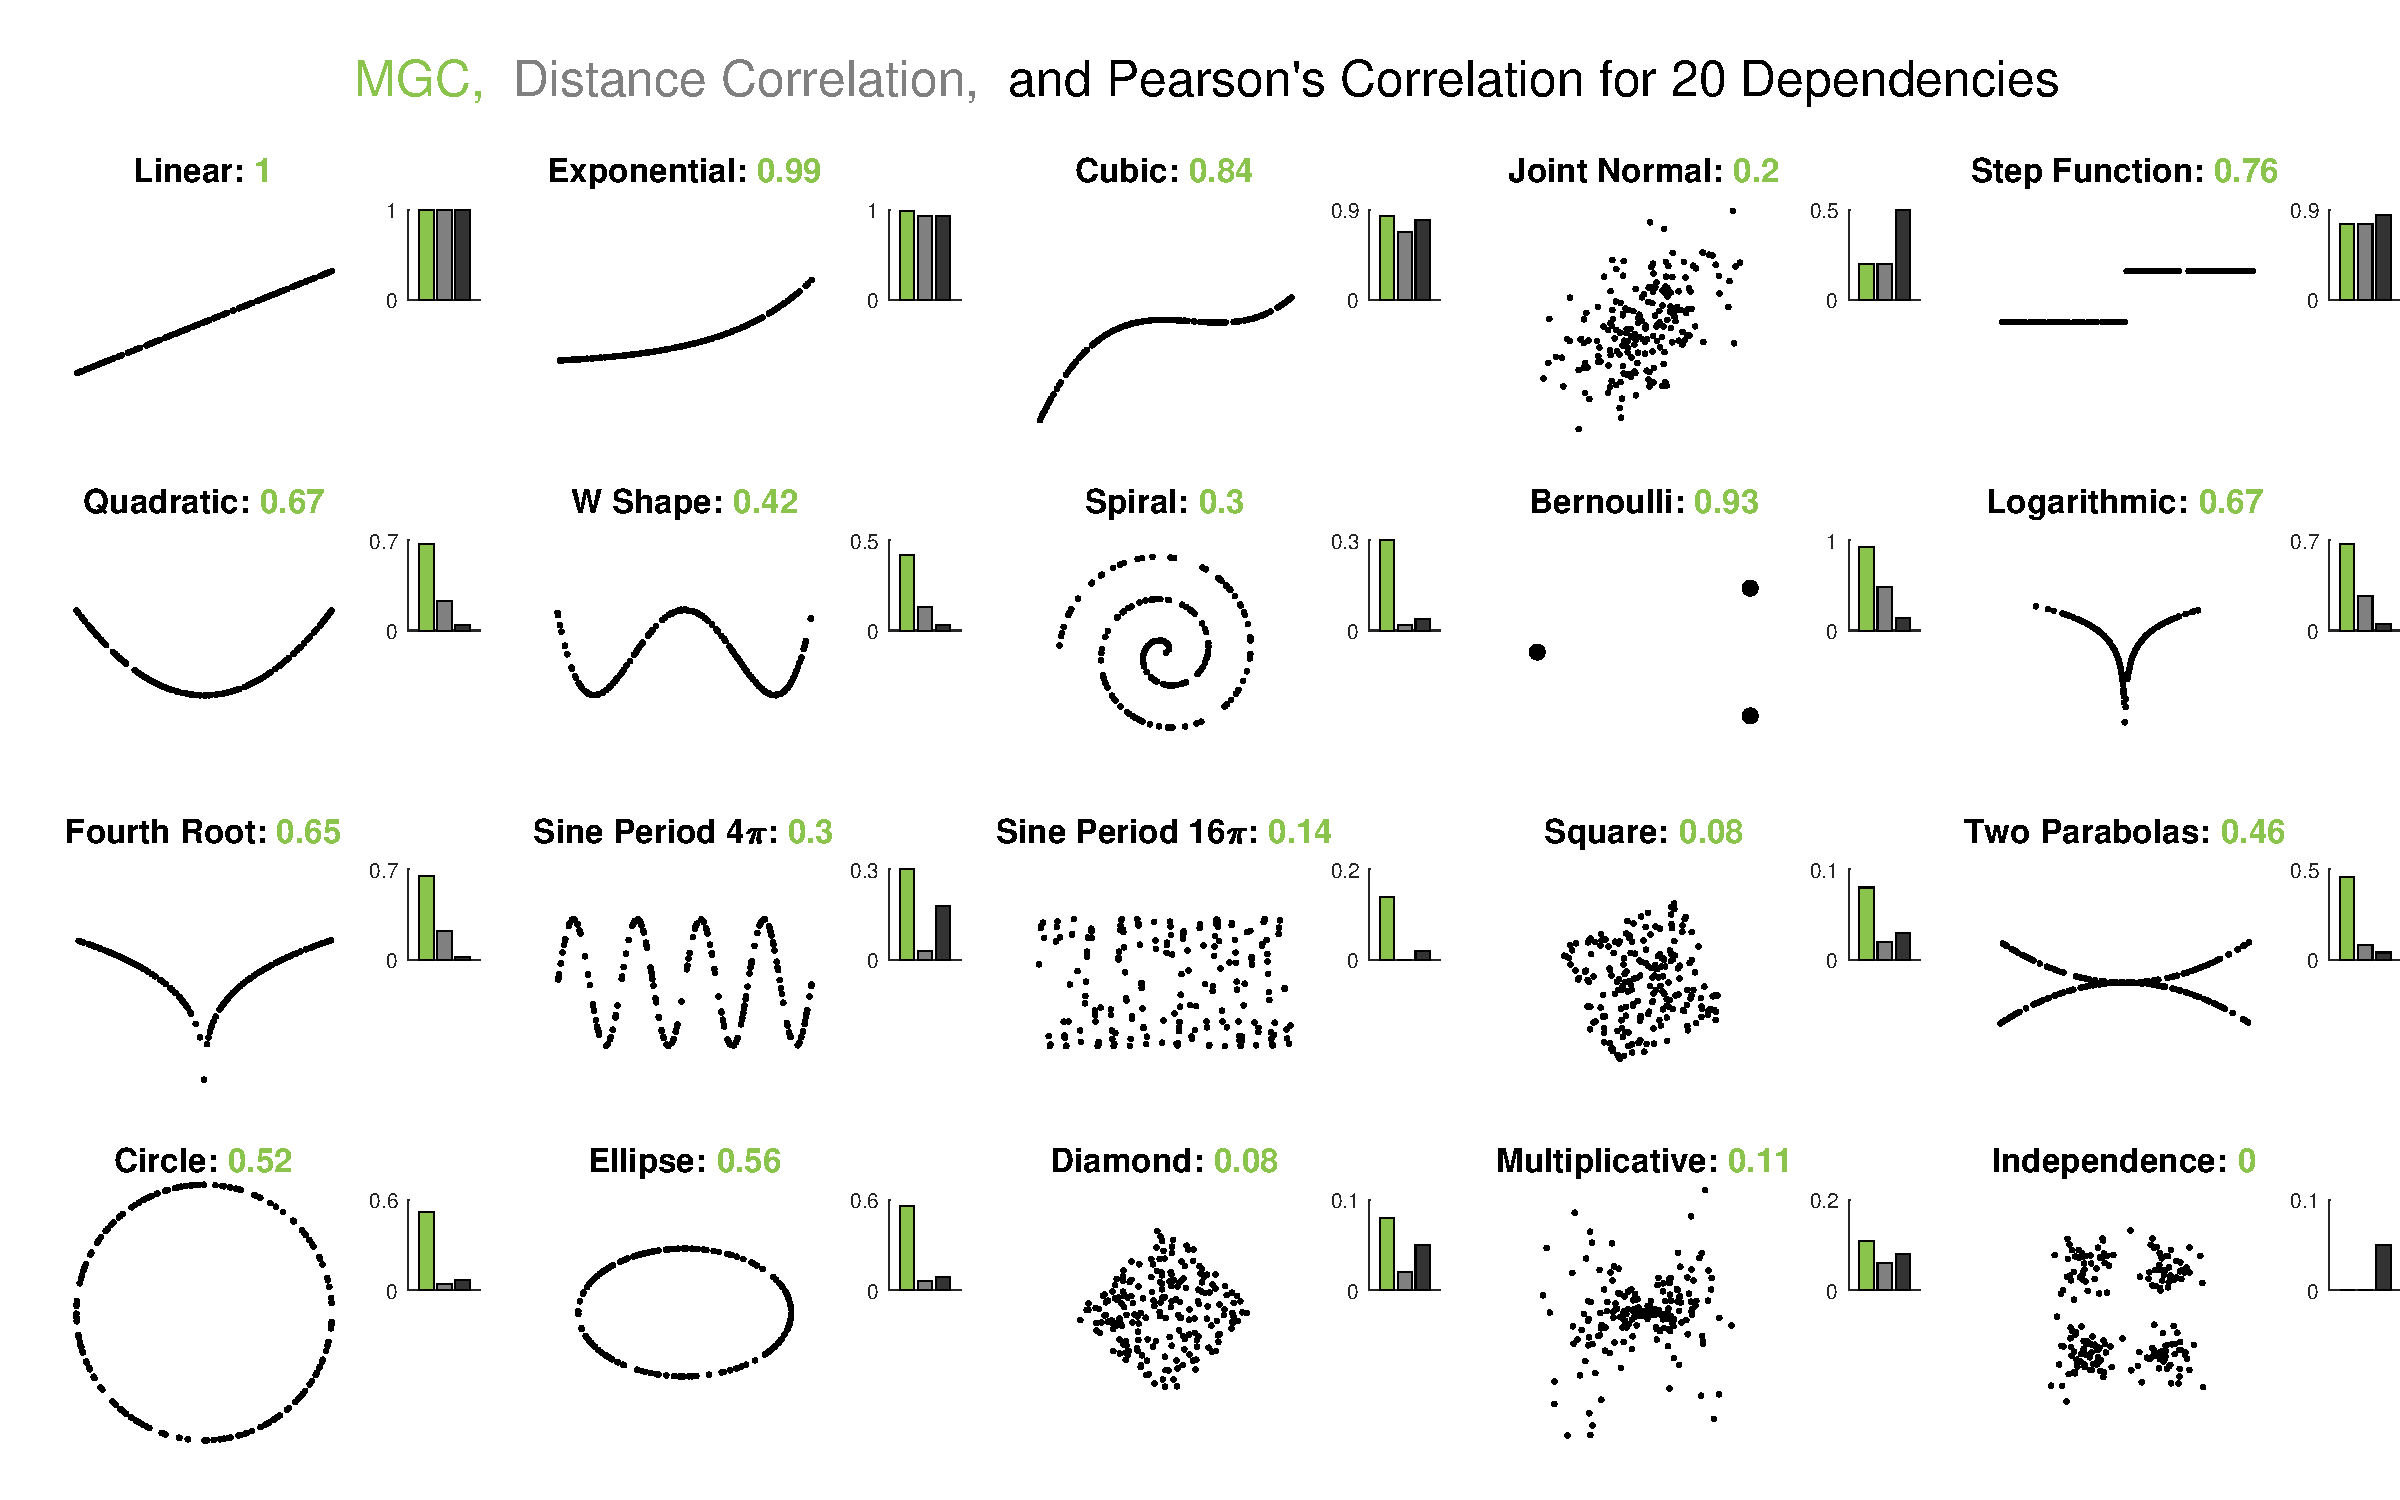
\includegraphics[width=1.0\textwidth]{FigSimVisual2}
	%\caption{Visualization of $\mbx$ vs $\mby$ for the $20$ dependencies at $p=1$ and $n=50$, and compute sample \Mgc~/ DCorr / absolute Pearson's correlation for each.}
	\label{f:dependencies}
\end{figure}
\end{frame}

\begin{frame}{Testing Power: Linear vs Nonlinear}
Power is the probability of rejecting the null when the alternative is true.
\pause
\begin{figure}[!ht]
\centering
% \subfigure{
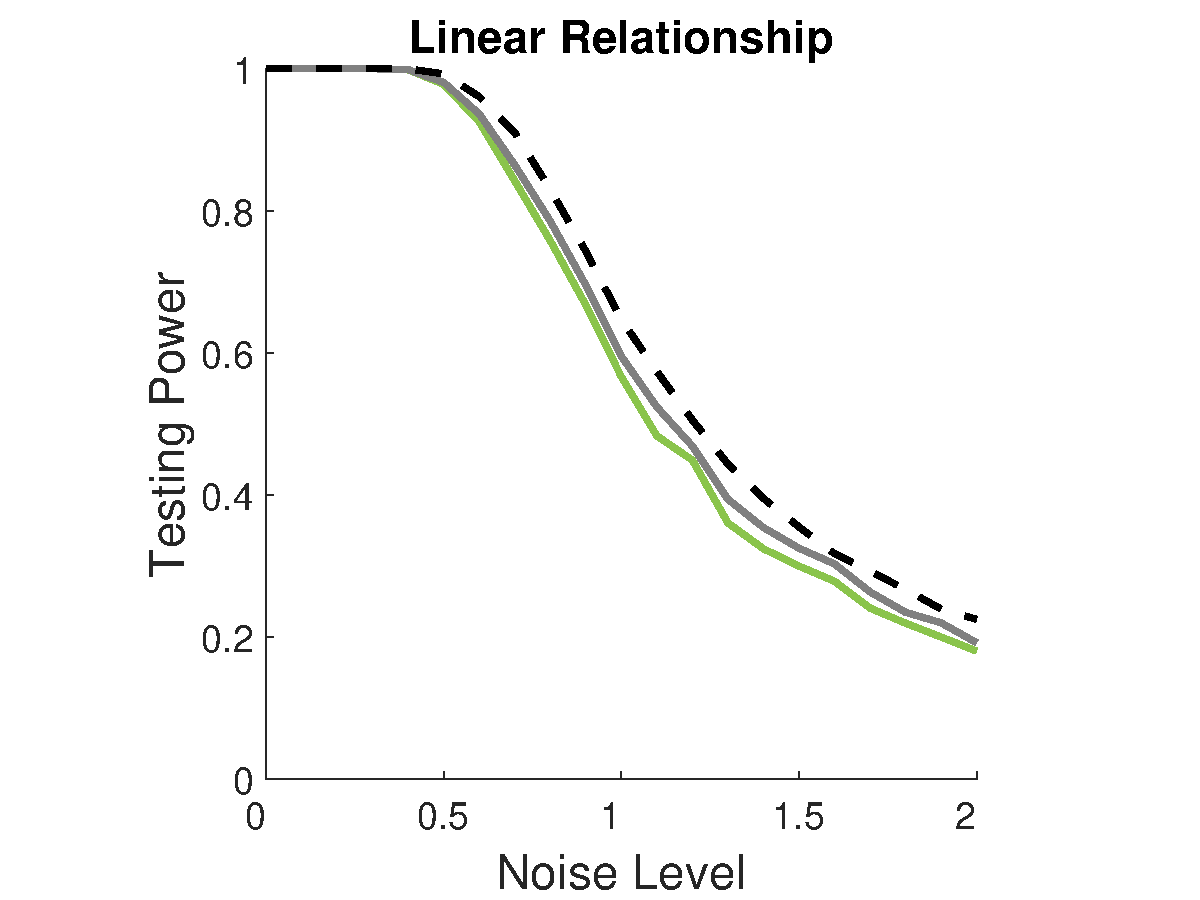
\includegraphics[width=0.5\textwidth,trim={1.5cm 0 0cm 0cm},clip]{FigNoiseT1}
% }
% \subfigure{
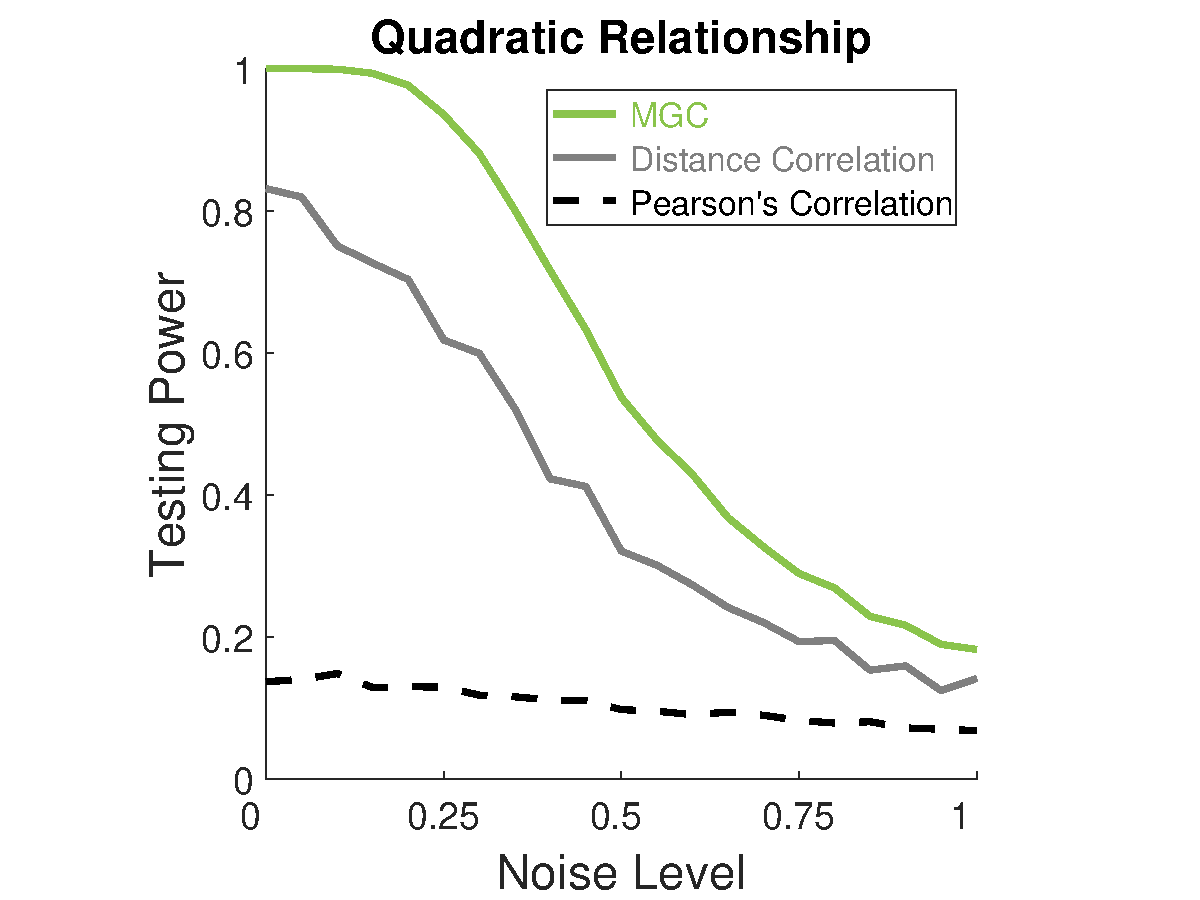
\includegraphics[width=0.5\textwidth,trim={1.5cm 0 0cm 0cm},clip]{FigNoiseT6}
% }
  %\caption{Comparing the power of \Mgc, distance correlation, and Pearson's correlation for testing noisy linear relationship, and noisy quadratic relationships at $p=1$ and $n=50$. Under linear relationship, all three of them are almost the same with Pearson's correlation being negligibly better; while under quadratic relationship, \Mgc~is clearly the best. \textbf{\Mgc~almost loses none in linear / gaussian setting while gains enormously in general dependency setting.}
\label{f:noise}
\begin{align*}
& n=30, p=q=1, \\
& X \sim Uniform(-1,1),\\
& \epsilon \sim Normal(0, noise), \\
& Y=X+\epsilon \mbox{ and } Y=X^{2}+\epsilon.
\end{align*}
\end{figure}
\end{frame}

%\begin{frame}{1D Simulation Powers}
%\begin{figure}[htbp]
%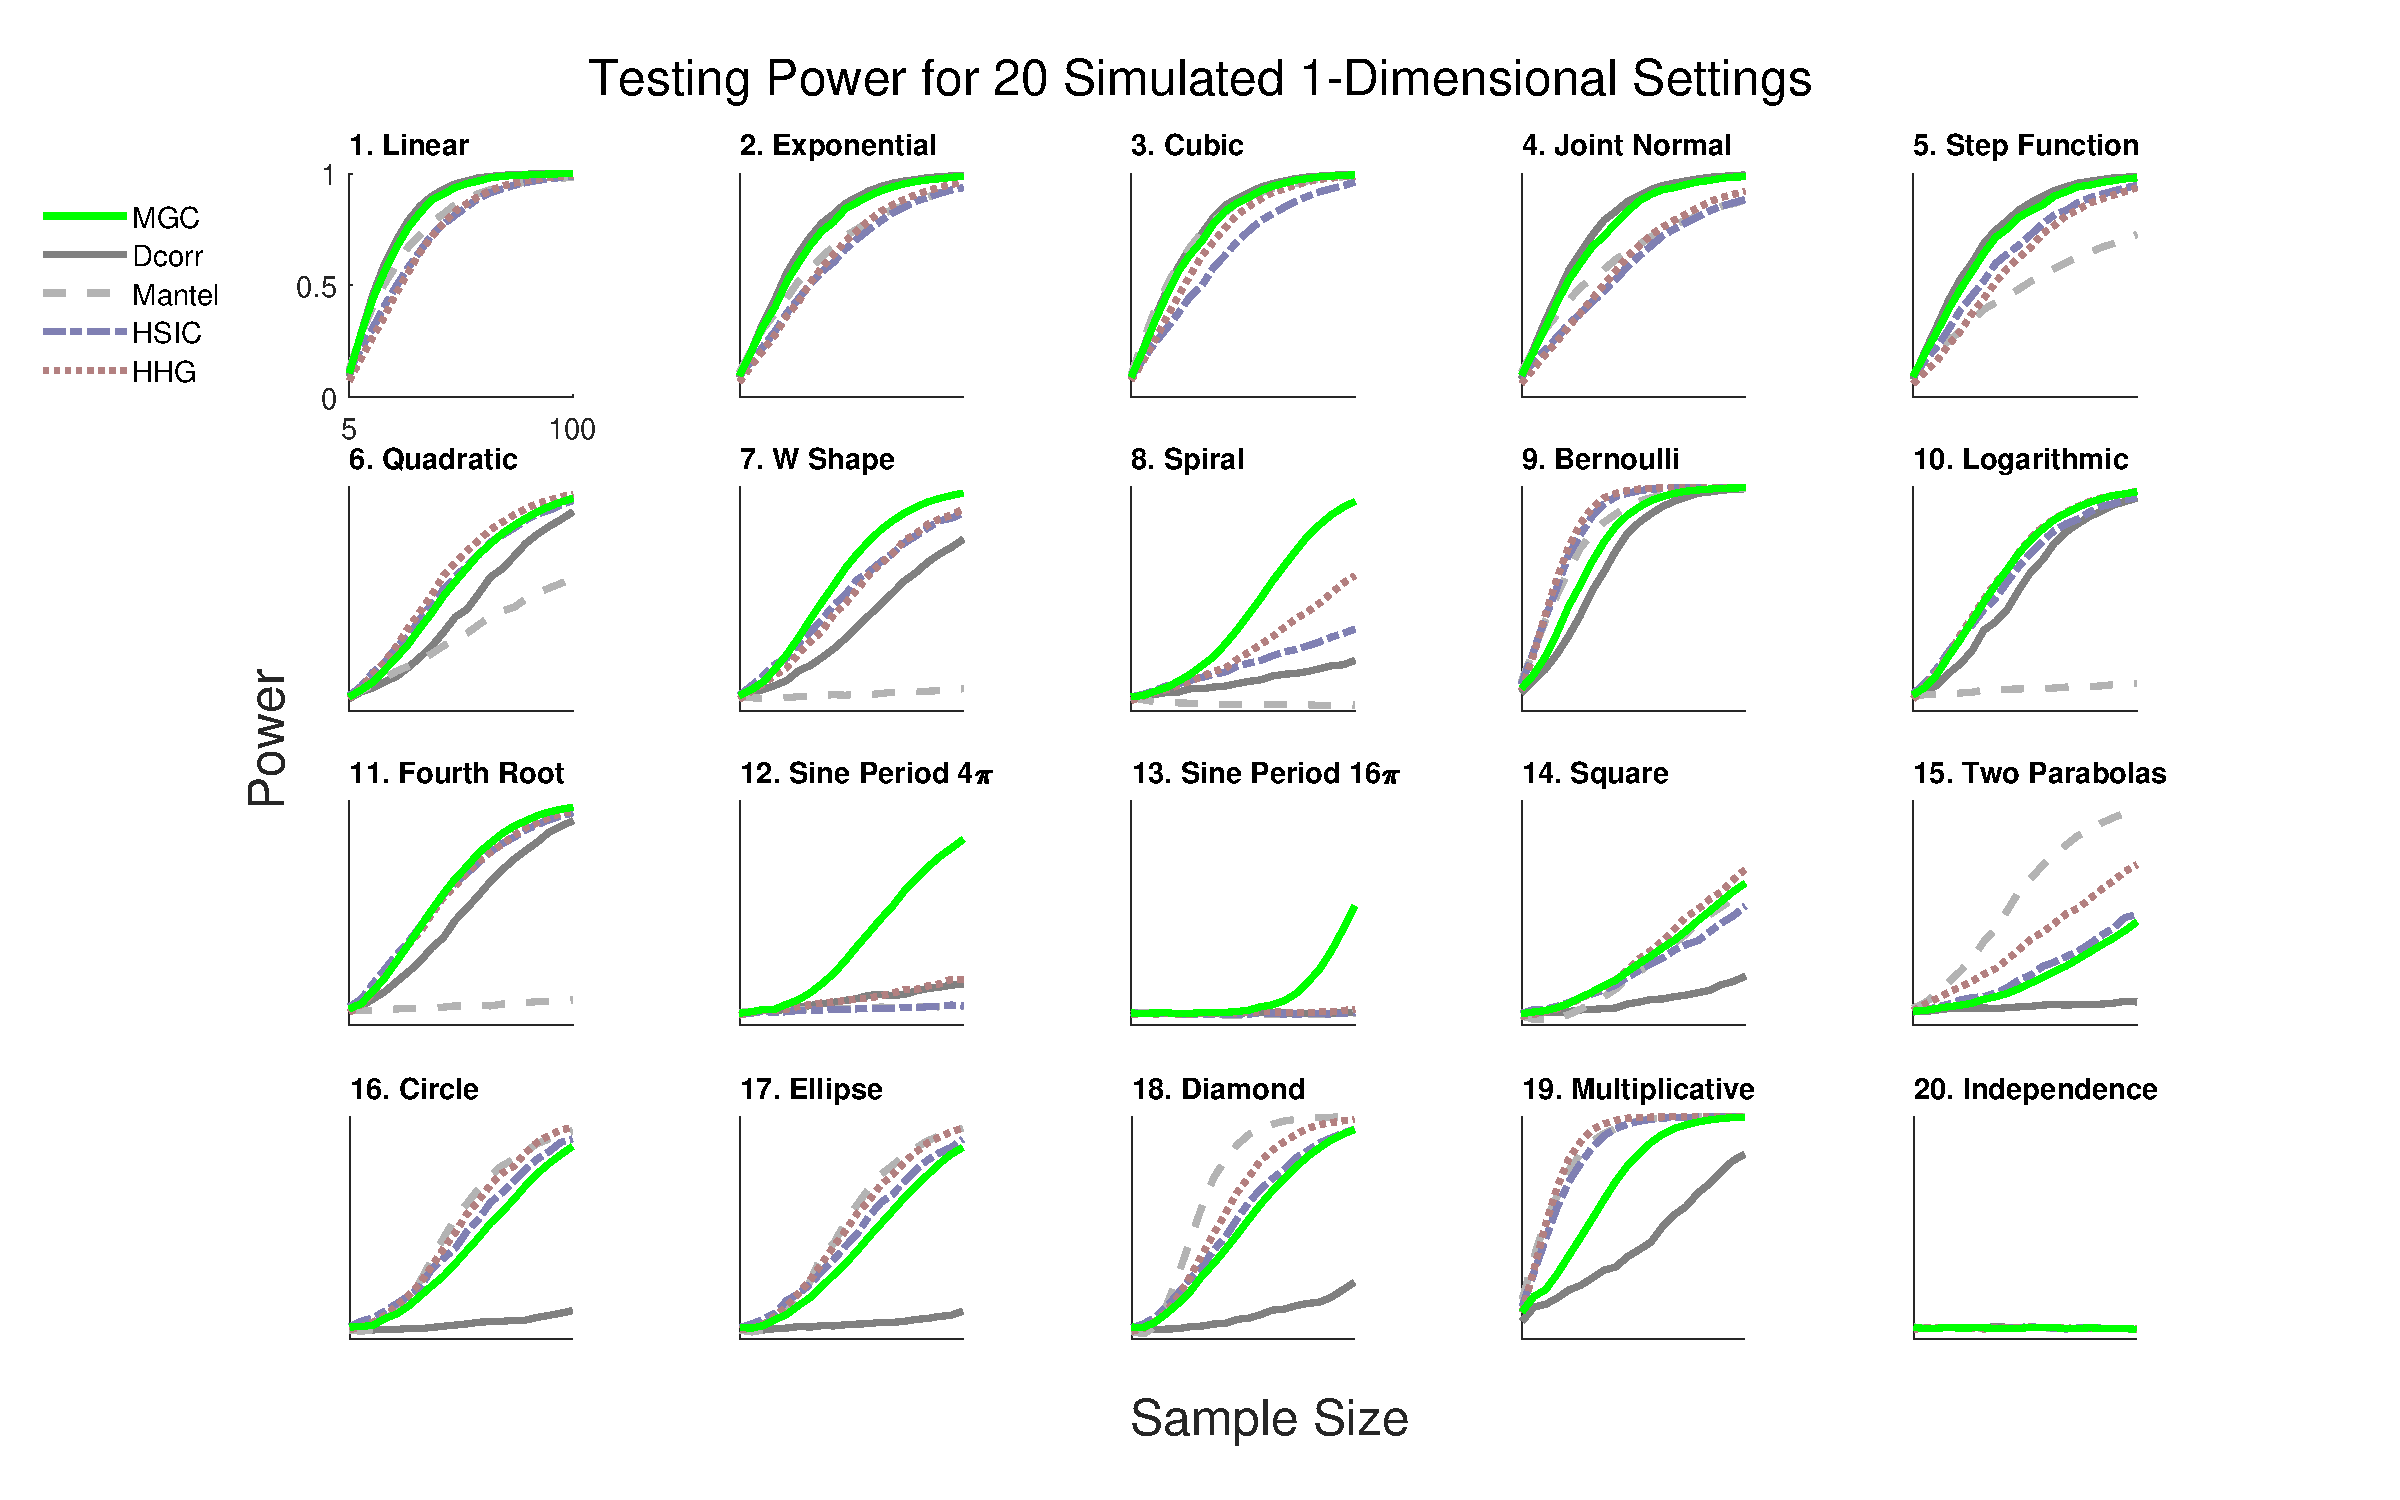
\includegraphics[width=0.9\textwidth]{Fig1DPowerAll}
%\caption{
%Powers of different methods for $20$ different one-dimensional dependence structures for increasing sample size.}
%\end{figure}
%\end{frame}

%\begin{frame}{HD Simulation Powers}
%\begin{figure}[htbp]
%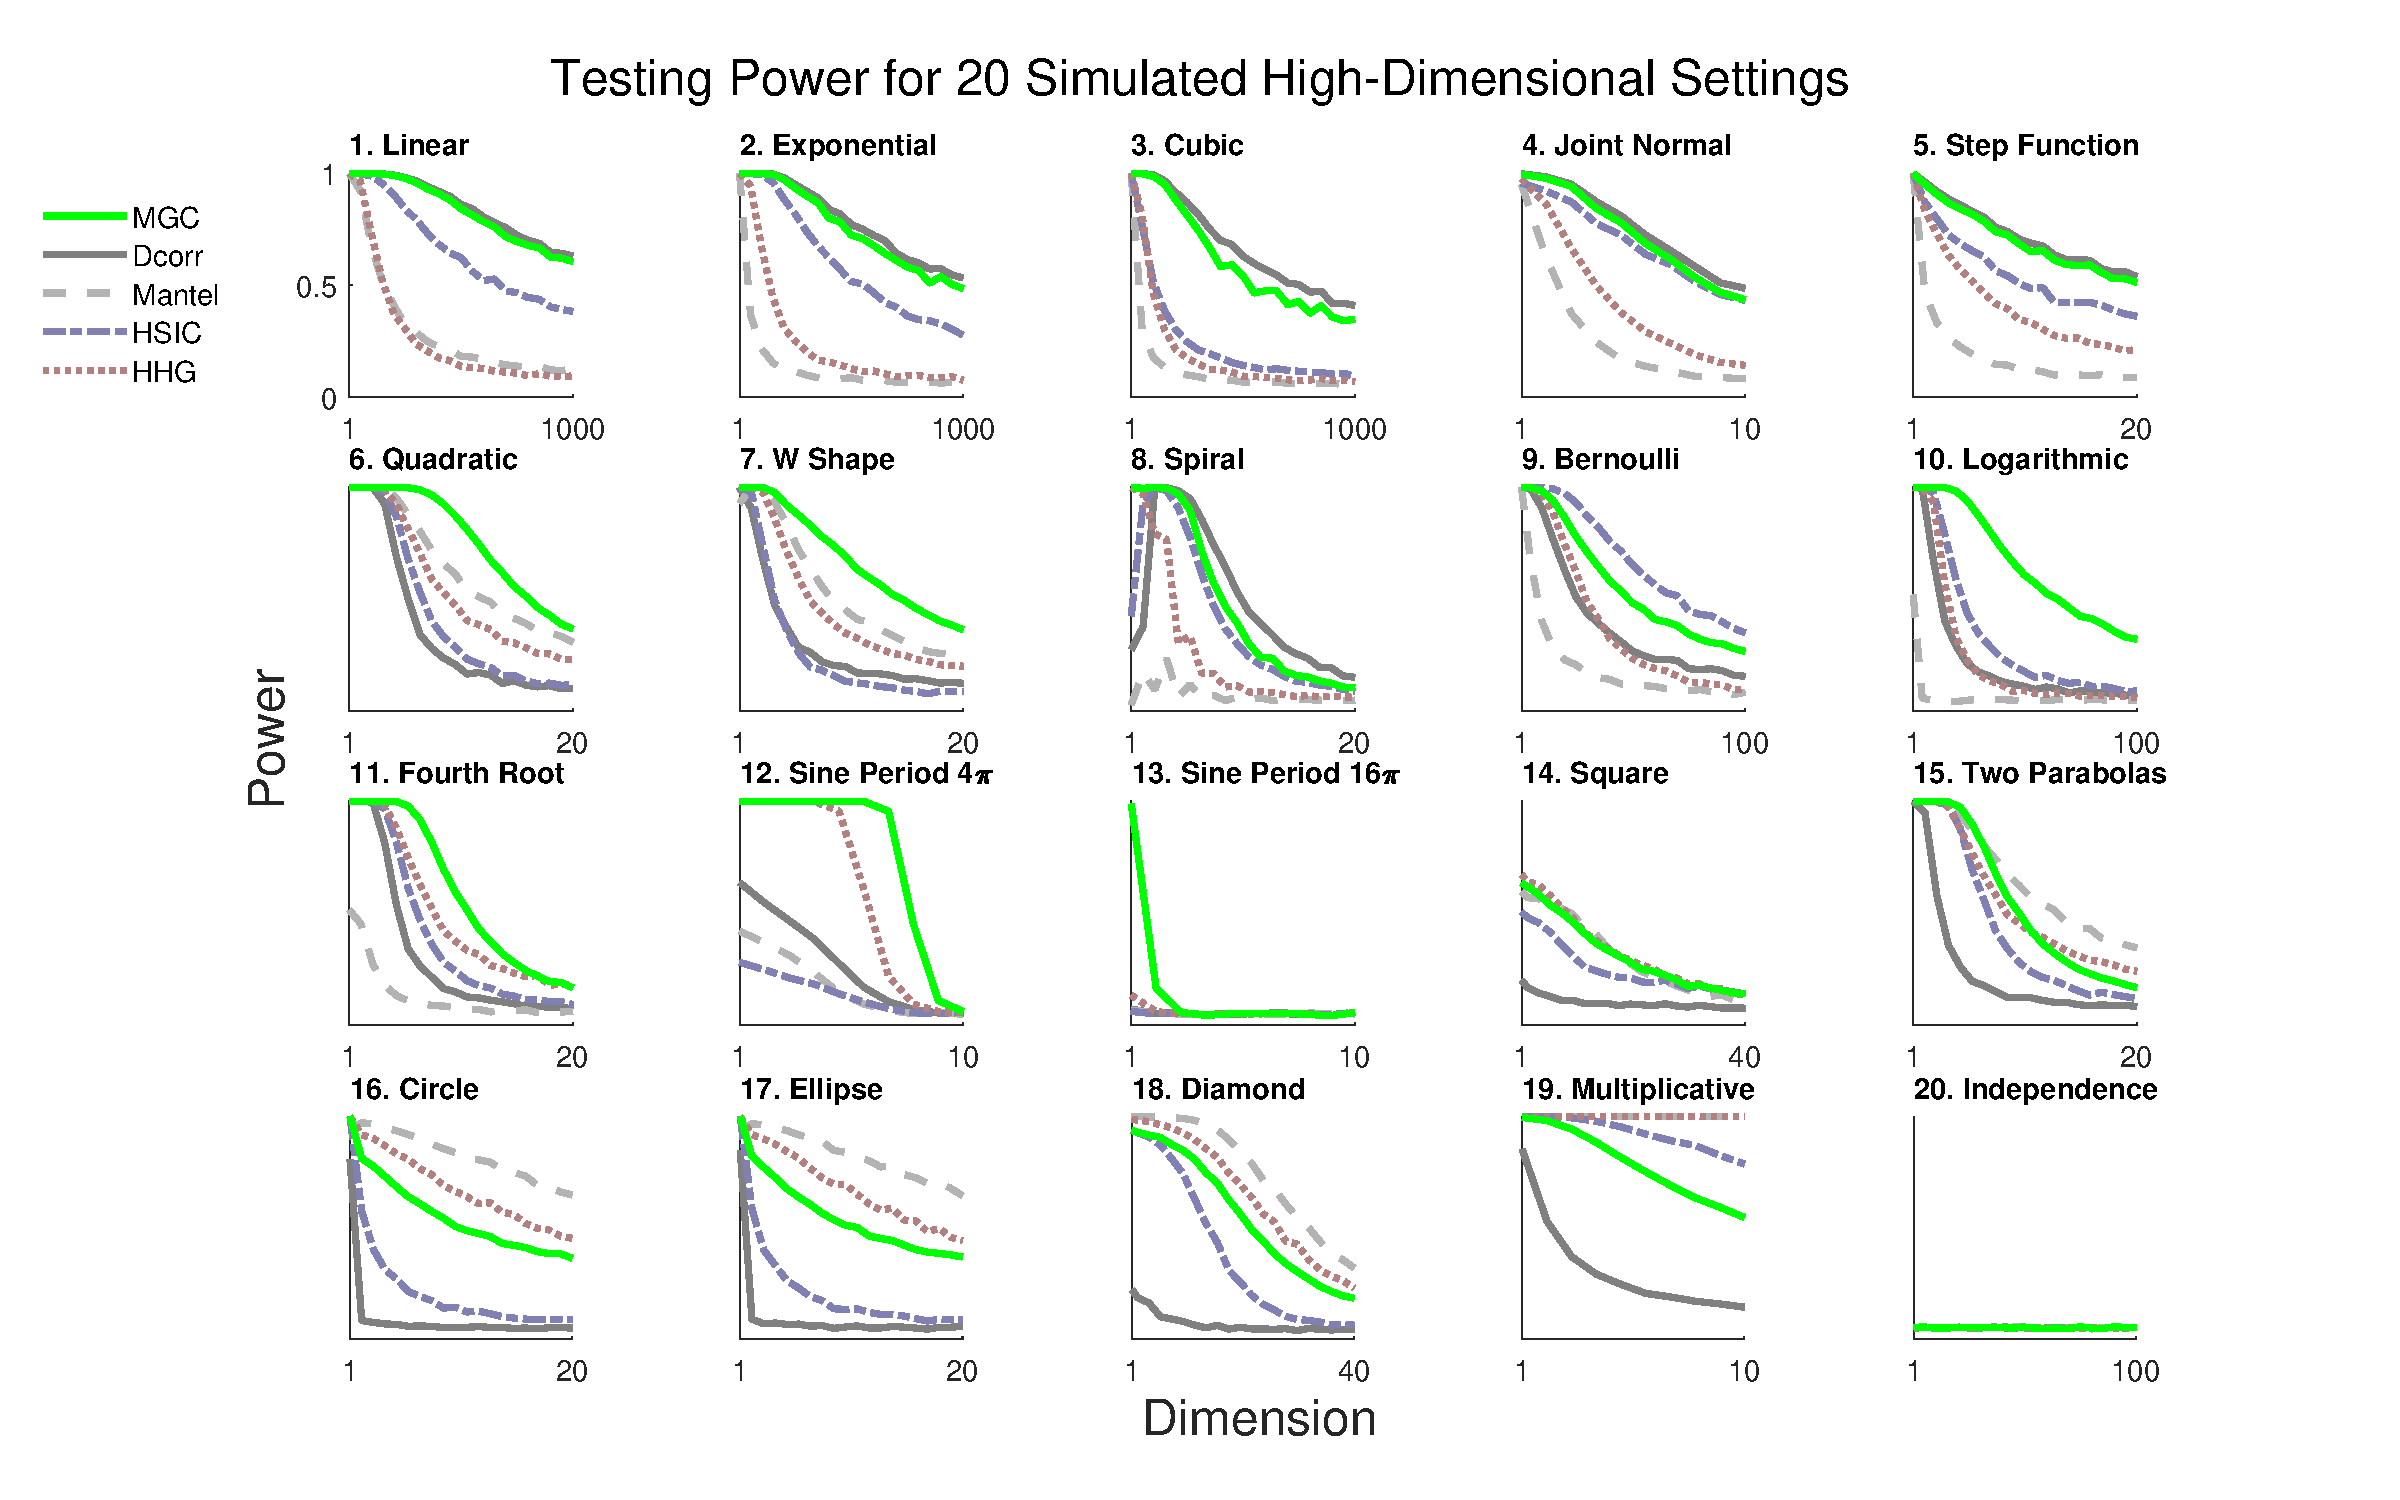
\includegraphics[width=0.9\textwidth]{FigHDPowerAll}
%\caption{
%Powers of different methods for $20$ different increasing-dimensional dependence structures, at $n=100$ and dimensionality increasing from $1$ onwards.}
%\end{figure}
%\end{frame}

%\begin{frame}{Relative Power in 1D}
%\pause
%\begin{figure}[!ht]
%\centering
% \subfigure{
%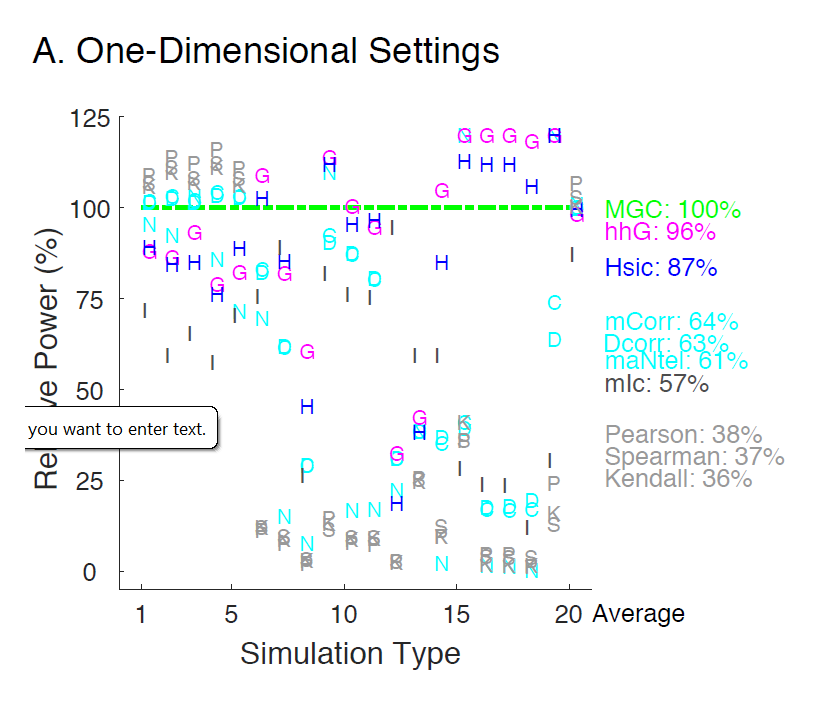
\includegraphics[width=0.75\textwidth,trim={0cm 0.2cm 0cm 0.3cm},clip]{Fig1DPowerSummary.png}
% }
% \subfigure{
%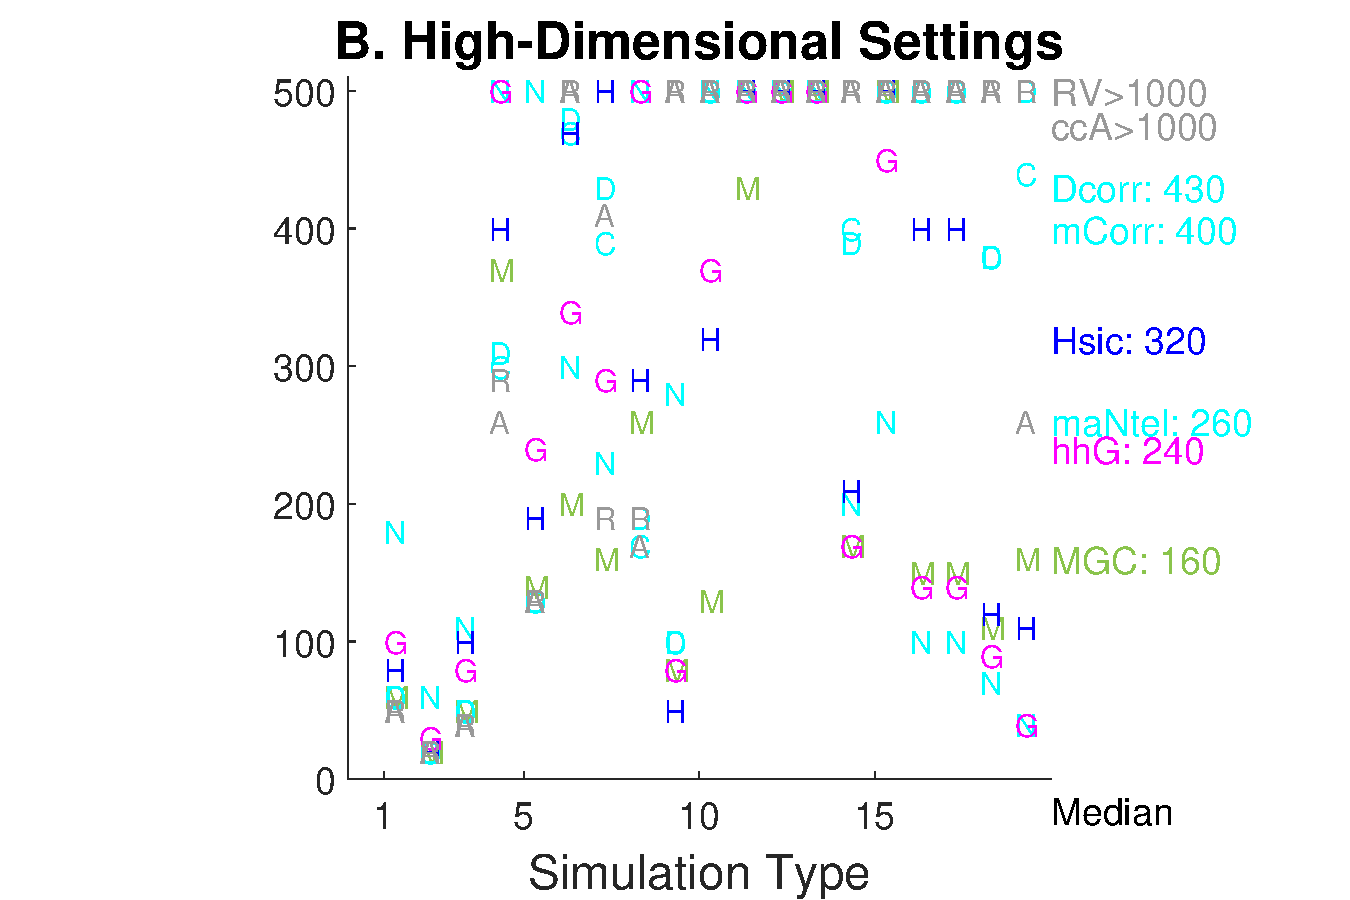
\includegraphics[width=0.99\textwidth,trim={2cm 0 0cm 0cm},clip]{FigHDPowerSummarySize}
% }
  %\caption{Required sample size of \Mgc~to achieve a power of $85\%$ in 1D and 10D at type 1 error level $5\%$, for each of the $20$ dependencies (except type 20 independent). The median size is reported in the far right column, and \Mgc~is overall the most superior method.}
%\label{f:Summary1}
%\end{figure}
%\end{frame}

%\begin{frame}{Relative Power in HD}
%\pause
%\begin{figure}[!ht]
%\centering
% \subfigure{
%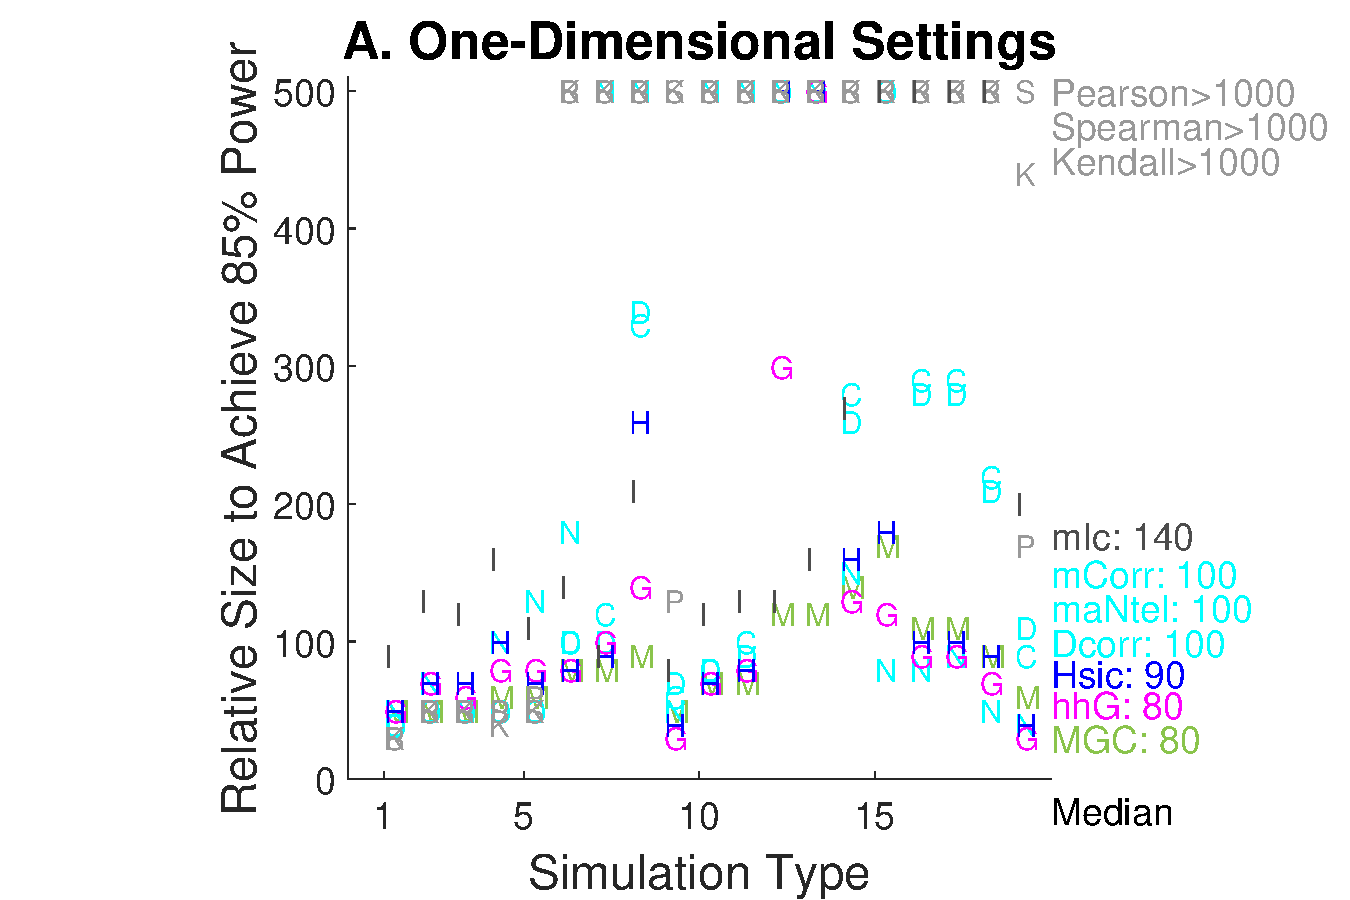
\includegraphics[width=0.99\textwidth,trim={2cm 0 0cm 0cm},clip]{Fig1DPowerSummarySize}
% }
% \subfigure{
%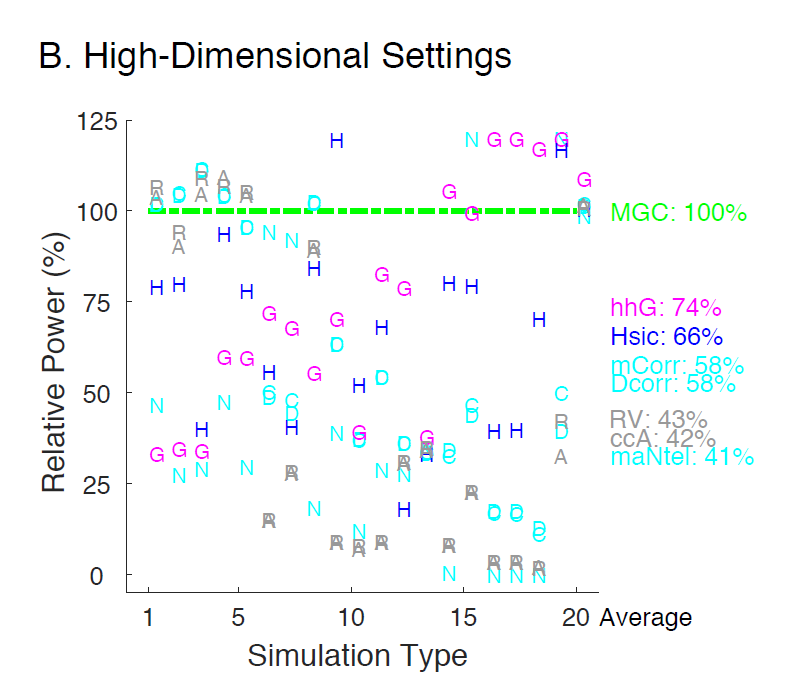
\includegraphics[width=0.75\textwidth,trim={0cm 0cm 0cm 0.5cm},clip]{FigHDPowerSummary.png}
% }
  %\caption{Required sample size of \Mgc~to achieve a power of $85\%$ in 1D and 10D at type 1 error level $5\%$, for each of the $20$ dependencies (except type 20 independent). The median size is reported in the far right column, and \Mgc~is overall the most superior method.}
%\label{f:Summary2}
%\end{figure}
%\end{frame}

\begin{frame}{Required Sample Size}
\pause
Required sample size $N_{\alpha,\beta}(c)$ to achieve a power of $\beta$ at type 1 error level $\alpha$ using a statistic $c$. We compute the required sample size $N_{\alpha=0.05,\beta=0.85}(c)$: \\
\medskip
\pause
in linear relationship, $40$ for all three methods; \\
in quadratic relationship, $80$ for \Mgc, $180$ for Dcorr, and $>1000$ for Pearson.\\

\medskip
\pause
Next we compute the size for each simulation, and summarize by the median over close-to-linear (type 1-5) and strongly non-linear relationships (type 6-19). \\

\medskip
\pause
We consider univariate (1D) and multivariate (10D) cases.\\ %Traditional linear correlations (Pearson/RV/CCA/ Spearman/Kendall) always perform the best in monotone simulations, so are the distance-based methods like Dcorr and \Mgc; HHG and HSIC are slightly worse, while MIC and Mantel are the worst. For non-monotone dependencies, traditional correlations fail to detect the existence of dependencies, while \Mgc~is the best approach followed by HHG and HSIC.
\end{frame}

\begin{frame}{Median Size Table}
\begin{tabular}{|l||c|c|c|c|}
\hline
Testing Methods & 1D Lin & 1D Non-Lin & 10D Lin & 10D Non-Lin   \\
\hline
%  Oracle \Mgc  & \textbf{50}  & 60 & \textbf{70} & \textbf{135} \\
% \hline
 \textcolor{UniOrange}{MGC}  & \textbf{50}  & \textbf{90} & 60 & \textbf{165} \\
\hline 
 Dcorr & \textbf{50}  & 250 & 60 & 515 \\
%\hline
% Mantel & 70  & 180 & 165 & 270\\
\hline
Pearson / RV / CCA & \textbf{50}  & $>$1000 & \textbf{50} & $>$1000 \\
\hline
 HHG & 70  & \textbf{90} & 100 & 315  \\
\hline
HSIC & 70  & 95 & 100 & 400 \\
%\hline
%Spearman & \textbf{50}  & n/a & $>$1000 & n/a \\
%\hline
%Kendall & \textbf{50}  & n/a & $>$1000 & n/a \\
\hline
MIC & 120  & 180 & n/a & n/a \\
%\hline
%CCA & \textbf{50}  & \textbf{50} & $>$1000 & $>$1000 \\
\hline
\end{tabular}
\end{frame}

\begin{frame}{Extracting Signal Brain Region from fMRI images}
\pause
We consider predicting the site and sex based on functional magnetic resonance image (fMRI) graphs. Two datasets used are SWU4 and HNU1, which have $467$ and $300$ samples respectively. \\
\medskip

Each sample is an fMRI scan registered to the MNI152 template using the Desikan altas, which has $70$ regions. They are transformed to graph structure using the NeuroData’s MRI Graphs pipeline \footnote{\url{https://github.com/neurodata/ndmg}}.
\medskip

We compute the dependency measure between each brain region and sex. Rank the brain region via magnitude of the measure, and include all significant ($p-val<0.05$) brain regions. Then run leave-one-out cross validation with $K$-Nearest Neighbor classifier to verify the results. Repeat it for the site property.
%Subsequent literature searches reveal that neurogranin is a potentially valuable biomarker because it is exclusively expressed in brain tissue among normal tissues and has not been linked with any other cancer type.

%\pause
%\medskip
%More details and other real data experiments can be found in \cite{ShenEtAl2016}.
\end{frame}

%\begin{frame}{P-value of Each Feature}
%\pause
%\begin{figure}[htbp]
%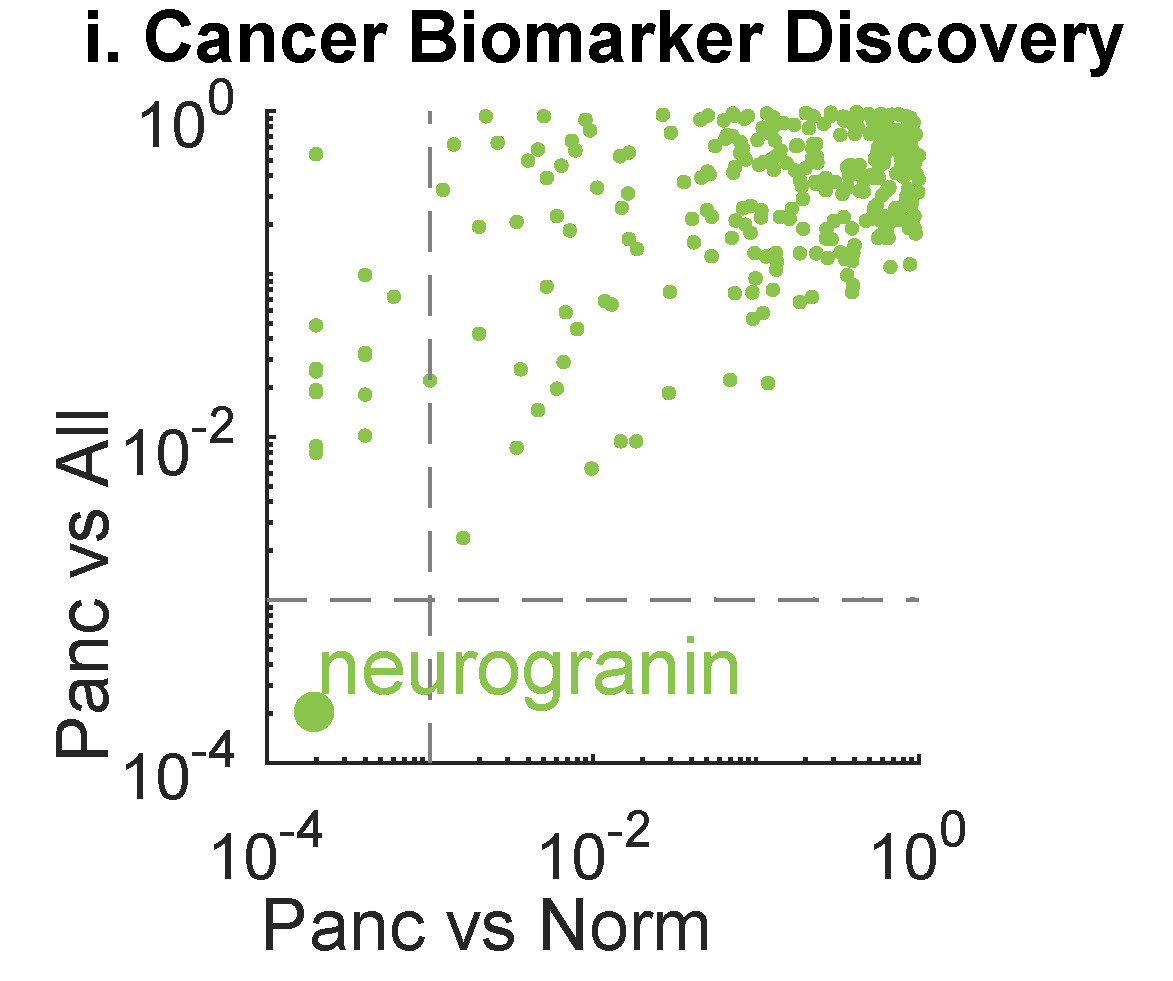
\includegraphics[width=0.6\textwidth]{FigReal1.png}
%\caption{X-axis is the p-value of each peptide between normal and pancreatic. Y-axis is the p-value between pancreatic and all other types. \Mgc~uniquely identifies Neurogranin.}
%\label{f:realA}
%\end{figure}
%\end{frame}

\begin{frame}
\begin{figure}[!ht]
	\centering
	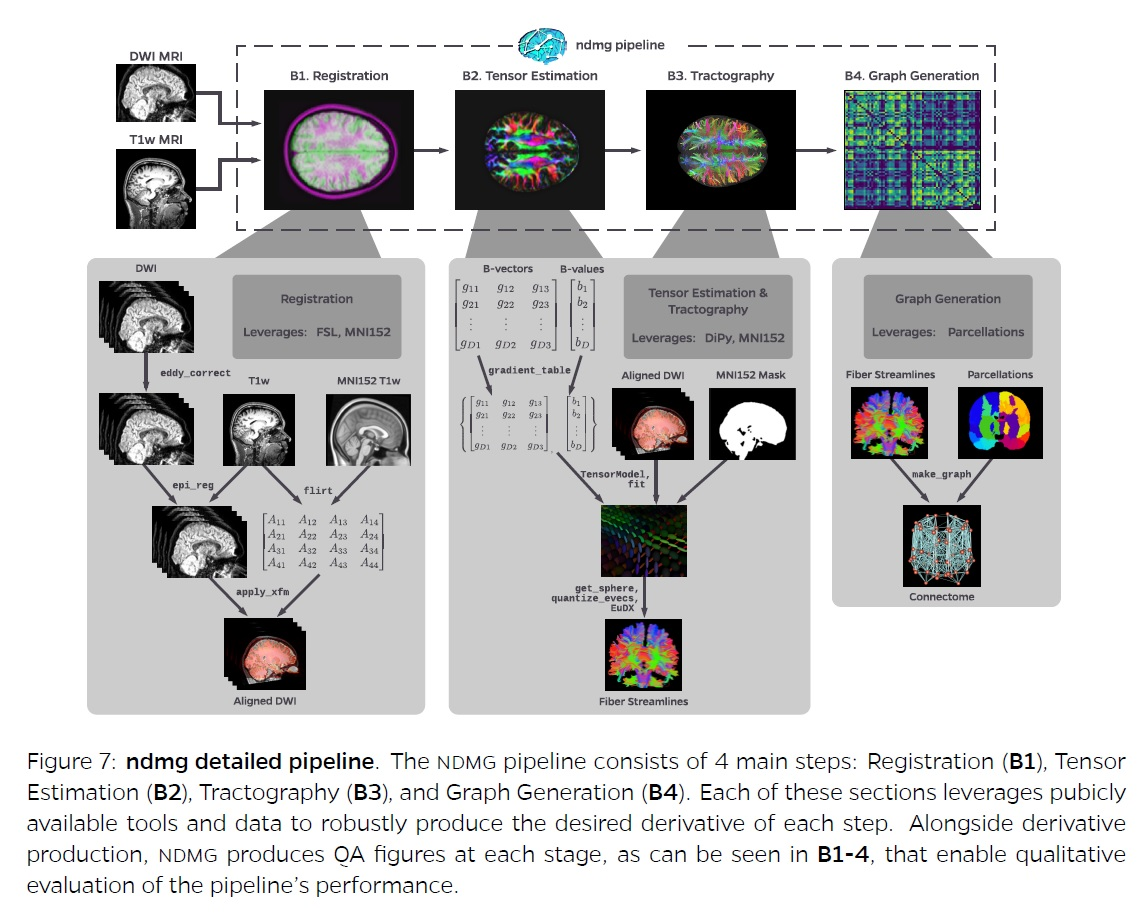
\includegraphics[width=4.3in]{brain0.jpg}
	\label{fig:study}
\end{figure}
\end{frame}

\begin{frame}
\begin{figure}[!ht]
	\centering
	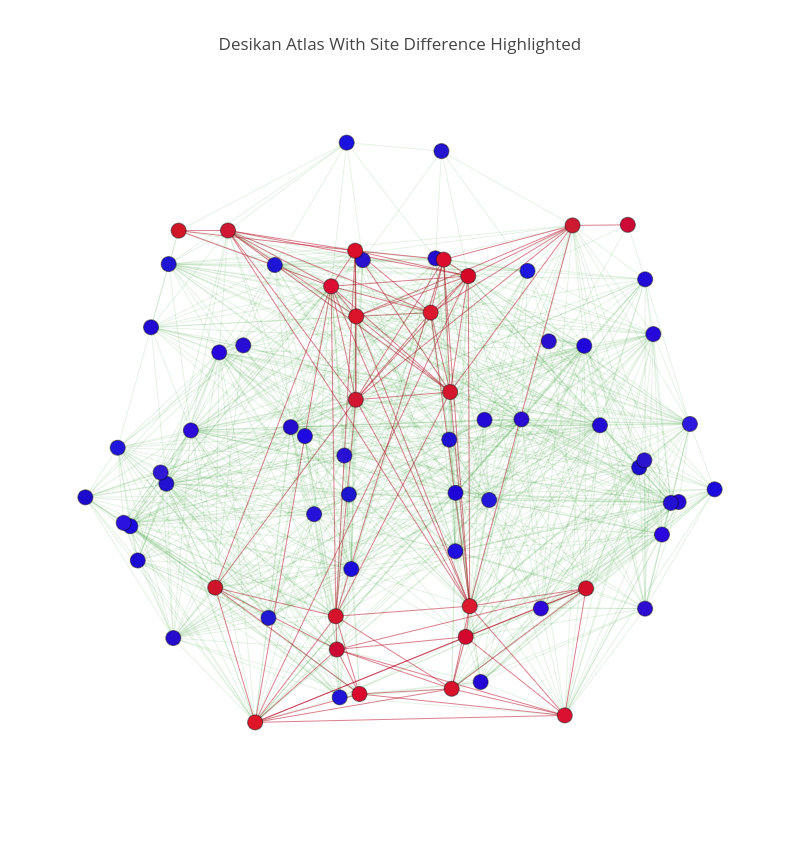
\includegraphics[width=3.5in]{brain.png}
	\label{fig:study}
\end{figure}
\end{frame}

\begin{frame}
\begin{figure}[!ht]
	\centering
	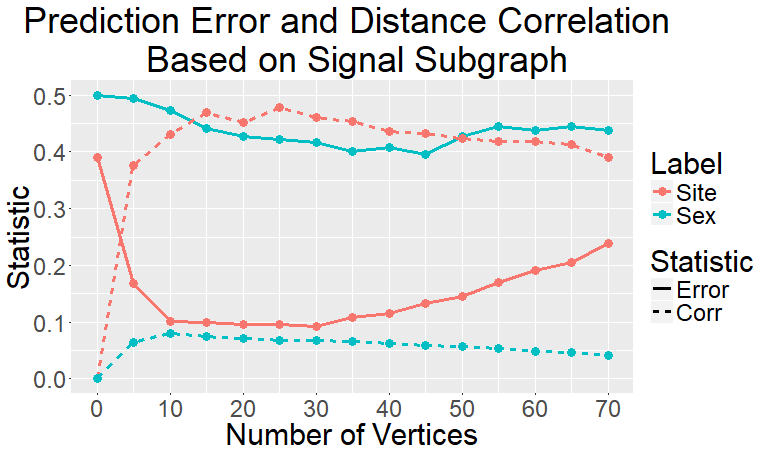
\includegraphics[width=3.5in]{batch_sex_cor_error.png}
	\label{fig:study}
	\caption{A total of $22$ regions are recognized for site difference, which maximizes the MGC statistic and almost minimizes the leave-one-out cross validation error. It is no longer the case for sex, for which neither the MGC nor the error are too significant for any size of subgraph.}
\end{figure}
\end{frame}

\section{Summary}
\begin{frame}{Summary}
\pause
Distance-based correlation is valid and universally consistent for testing independence. \Mgc~utilizes the locality principle to achieve better testing power and sheds insight into the dependency structure.

\pause
\medskip
\begin{itemize}[<+->]
\item Using a proper distance or kernel ensures the universal consistency.
\item Compute all local correlations iteratively and finds the optimal one can help the testing power when sample size is limited.
\item The optimal scale gives information on linear vs nonlinear dependency.
\item It can be used in a variety of applications to replace the Pearson's correlation.
\end{itemize}
%\pause
%\medskip
%In this talk we went over the tip of the iceberg; there are a lot more fascinating details and applications in the manuscripts.
\end{frame}

\begin{frame}{Advantages of \Mgc}
\pause
1. Performant under any joint distribution of finite second moments:
\pause
\begin{itemize}[<+->]
\item Equals $0$ asymptotically if and only if independence.
\item \textcolor{UniOrange}{Amplify the dependency signal while mostly avoiding the sample bias.} 
\item Superior finite-sample performance over all benchmarks, against linear / nonlinear / noisy / high-dimensional relationships. 
\end{itemize}

\pause
\medskip
2. It works for:
\pause
\begin{itemize}[<+->]
\item Low- and high-dimensional data.
\item Euclidean and structured data (e.g., images, networks, shapes).
\item Any dissimilarity / similarity / kernel matrix.
\end{itemize}

\pause
\medskip
3. Intuitive to understand and efficient to implement in $\mathcal{O}(n^2 log n)$.

%\pause
%\medskip
%MGC shares the same intrinsic idea as in nonlinear embedding, random forest, multiple kernel learning, deep learning.
\end{frame}

\begin{frame}{Some Recent Advances in Computation}
In practice:
\pause
\medskip
\medskip

1. Distance correlation and MGC can now be tested without resorting to permutation (similar to Pearson's t-test).
\pause
\medskip
\medskip

2. When $p=q=1$ and using Euclidean distance, there is a special fast implementation of distance correlation. The running time becomes $O(n \log n)$ and storage requirement becomes $O(n)$, making it ideal and scalable to millions and billions of observations. (less than $10$ seconds for $1$ million observations on a standard PC using Matlab)
\pause
\medskip
\medskip

Thus when $n$ is small (say less than a few thousands), \Mgc~is the better choice; whereas distance correlation can better handle extremely large data.
\end{frame}

\begin{frame}{Open Source Packages}
Python package in \url{https://github.com/neurodata/mgcpy/} and forthcoming in scikit-learn\\
\bigskip
R package in \url{https://github.com/neurodata/MGC/} and CRAN\\
\bigskip
Matlab code \url{https://github.com/neurodata/mgc-matlab}
\end{frame}
%\begin{frame}{Current Works}
%\pause
%\begin{itemize}[<+->]
%\item The sample method, algorithmic details, simulation advantages and real applications are demonstrated in [\textit{Shen et al.(2017a)}]\cite{ShenEtAl2016}.
%\item Population \Mgc~and most mathematical properties appear in [\textit{Shen et al.(2017b)}]\cite{ShenEtAl2018}.
%\item \Mgc~is infused with diffusion maps for testing between graph vertices and attributes [\textit{Lee et al.(2017)}]\cite{Lee2017}.
%\item \Mgc~is utilized for iterative signal subgraph extraction in [\textit{Wang et al.(2018)}]\cite{Wang2017}.
%\if1\blind{
%\item The local correlation map characterizes the dependency structure \cite{ShenEtAl2019}.
%\item \Mgc~is an ideal choice for K-sample testing \cite{ShenEtAl2019b}.
%}\fi
%\end{itemize}
%\end{frame}

%\begin{frame}{Future Directions}
%\pause
%\begin{itemize}[<+->]
%\item Feature selection / dimension reduction.
%\item Magnitude of \Mgc~versus prediction and classification error.
%\item Better classification / regression in multiple graph setting.
%\item Rank or Kernel \Mgc; interpretation of the optimal local scale under RKHS framework.
%\item Relative efficiency among \Mgc, Dcorr, Mantel, and HSIC.
%\item Faster \Mgc~testing.
%, sub-sampling performance guarantee in big data, and approximated null distribution to derive p-value without permutation test.
%\item Real data applications.
%: neurodata vs phenotypes, genotypes vs phenotypes, social networks vs attributes, plane sensor data vs mechanical issue, etc.
%\end{itemize}
%\end{frame}
%\section{Method}
%\begin{frame}{Distance Matrices}
%\pause
%\textbf{Input:} Given pairs of observations $(x_{i},y_{i}) \in \Real^{p} \times \Real^{q}$ for $i=1,\ldots,n$, denote $X_{n}=[x_{1},\ldots,x_{n}]$ as the data matrix with each column representing one sample observation, and similarly $Y_{n}$. \\
%\pause
%\medskip
%\textbf{Distance Computation: } Let $\tilde{A}$ be the $n \times n$ Euclidean distance matrices of $X_{n}$:
%\begin{align*}
%\tilde{A}_{ij}=\|x_{i}-x_{j}\|_{2},
%\end{align*}
%and similarly $\tilde{B}$.\\

%\pause
%\medskip
%Alternatively, one can directly input two distance / dissimilarity matrices.
%For $p=q=1$, the sample Pearson's covariance equals  
%\begin{equation}
%cov(X,Y)=\frac{1}{n-1}\sum_{i=1}^{n}(x_{i}-\overline{x})(y_{i}-\overline{y}).
%\end{equation}
%with $\overline{x}$ and $\overline{y}$ being the sample mean.

%\pause
%\medskip
%The variance can be similarly defined as $cov(X,X)$ and $cov(Y,Y)$, and correlation follows as 
%\begin{equation}
%corr(X,Y)=\frac{cov(X,Y)}{\sqrt{cov(X,X) cov(Y,Y)}} \in [-1,1].
%\end{equation}

%The RV coefficient (or canonical correlation) generalizes the Pearson's correlation into dimensionality higher than $1$.
%\end{frame}

%\begin{frame}{Transforming the Distance Matrices}
% \pause
%\textbf{Centering:} Then we center $\tilde{A}$ and $\tilde{B}$ by columns, with the diagonals excluded:
%\begin{equation}
%\label{localCoef2}
 %   A_{ij}=
 %   \begin{cases}
 %     \tilde{A}_{ij}-\frac{1}{n-1}\sum_{s=1}^{n} \tilde{A}_{sj}, & \text{if $i \neq j$}, \\    
 %     0, & \text{if $i=j$};
 %   \end{cases}
%\end{equation}
%similarly for $B$. 

%\pause
%\medskip
%The distance covariance statistic by \textit{Szekely et al.(2007)} equals the mean of the entri-wise product of $A$ and $B^{T}$, i.e., 
%\begin{equation}
%dcov(X,Y)=\frac{1}{(n-1)^2}\sum_{i,j=1}^{n}A_{ij} B_{ji}.
%\end{equation}
%Similarly one can define distance variance, and then distance correlation in $[-1,1]$.
%While Multiscale Generalized Correlation (\Mgc) only consider local distances, i.e., calculate the correlation between two sparse matrices based on nearest-neighbor.
%\end{frame}

%\begin{frame}{Examples}
%A few examples of $\G$:
%\begin{itemize}[<+->]
%\item The Pearson's product-moment correlation coefficient by taking $a_{ij}=x_i$ and $b_{ij}=y_i$.
%\item The Spearman and Kendall's rank correlations by setting $a_{ij}$ to be $rank(x_i)-rank(x_j)$ and $sign(x_i-x_j)$ respectively.
%\item The Mantel coefficient [\textit{Mantel (1967)}]\cite{Mantel1967} by using $a_{ij}=|x_i-x_j|_{2}$ (i.e. Euclidean distance).
%\item The distance correlation [\textit{Szekely et al.(2007)}]\cite{SzekelyRizzoBakirov2007} by using the doubly-centered distance entries for $a_{ij}$ and $b_{ij}$.
%\item The modified distance correlation [\textit{Szekely and Rizzo (2013)}] \cite{SzekelyRizzo2013a} by slightly tweaking $a_{ij}/b_{ij}$ of dcorr.
%\end{itemize}
%\end{frame}

%\begin{frame}{Incorporating the Locality Principle}
%\pause
%\textbf{Ranking:} Define $\{R^{A}_{ij}\}$ as the ``rank'' of $x_i$ relative to $x_j$, that is, $R^{A}_{ij}=k$ if $x_i$ is the $k^{th}$ closest point (or ``neighbor'') to $x_j$, as determined by ranking the set $\{\tilde{A}_{1j},\tilde{A}_{2j},\ldots,\tilde{A}_{nj}\}$ by ascending order. Similarly define $R^{B}_{ij}$ for the $y$'s. 

%\pause
%\medskip
%For any $(k,l) \in [n]^2$, define the rank truncated matrices $A^{k}, B^{l}$, and the joint distance matrix $C^{kl}$ as
%\begin{align*}
%A_{ij}^{k} &=A_{ij} \mb{I}(R^{A}_{ij} \leq k), \\
%B_{ji}^{l} &=B_{ji} \mb{I}(R^{B}_{ji} \leq l), \\
%C^{kl}_{ij} &= A_{ij}^{k} \times B_{ji}^{l},
%\end{align*}
%where the subscript of $B$ is purposely switched.

%\pause
%\medskip
%When ties occur, minimal rank is used, e.g., if $\mby$ only takes two value, $R^{B}_{ij}$ takes value in $\{1,2\}$ only. We assume no ties for each of presentation.
%\end{frame}

%\begin{frame}{Local Distance Correlations}
%\pause
%\textbf{A Family of Local Correlations:} 
%Finally, we compute the sample local covariance, variance, and correlation between the sample observations $X_{n}$ and $Y_{n}$ as follows:
%\pause
%\begin{align*}
%dCov^{kl}(X_{n},Y_{n}) &= \E(C^{kl}_{ij})- \E(A^{k}_{ij})\E(B^{l}_{ij}),\\
%dVar^{k}(X_{n}) &=\E(A^{k}_{ij} A^{k}_{ji})- \E^2(A^{k}_{ij}), \\
%dVar^{l}(Y_{n}) &=\E(B^{l}_{ij} B^{l}_{ji})- \E^2(B^{l}_{ij}), \\
%dCorr^{kl}(X_{n},Y_{n}) &=dCov^{kl}(X,Y) / \sqrt{dVar^{k}(X) \cdot dVar^{l}(Y)}.
%\end{align*}
%for $k,l=1,\ldots,n$, and $\E(\cdot)=\frac{1}{n(n-1)}\sum_{i \neq j}^{n} (\cdot)$ denotes the diagonal-excluded sample mean of a square matrix. If $dVar^{k}(X_{n}) \cdot dVar^{l}(Y_{n}) \leq 0$, we set $dCorr^{kl}(X_{n},Y_{n})=0$ instead. 

%\pause
%\medskip
%There are a maximum of $n^2$ different local correlations. At $k=l=n$, $dCorr^{kl}(X_{n},Y_{n})$ equals the ``global'' distance correlation $dCorr(X_{n},Y_{n})$ by \textit{Szekely et al.(2007)}.
%\end{frame}

%\begin{frame}{MGC}
%\pause
%\textbf{MGC as optimal local correlation:} In $\{dCorr^{kl}(X_{n},Y_{n})\}$, we shall take the ``optimal'' local correlation as the \Mgc~statistic $\G^{*}(X_{n},Y_{n})$. 

%\pause
%\medskip
%However, directly taking the maximum local correlation $\max_{(k,l) \in [n]^2}\{dCorr^{k,l}(X_{n},Y_{n})\}$ will yield a biased statistic under independence, i.e., the maximum is always larger than $0$ in expectation even under independent relationship.

%\pause
%\medskip
%Instead, we take a smoothed maximum by:
%\begin{itemize}[<+->]
%\item Pick a threshold $\tau \geq 0$;
%\item Compute the largest connected component $R=\{(k,l)$ such that $dCorr^{kl}(X_{n},Y_{n})>\max\{\tau, dCorr^{nn}(X_{n},Y_{n})\} \}$;
%\item Within the significant region $R$, set $\GG^{*}(X_{n},Y_{n})=\max_{ (k,l) \in R} \{dCorr^{k,l}(X_{n},Y_{n})\}$;
%\item If the number of elements in $R$ is less than $2n$, or the $\GG^{*}(X_{n},Y_{n})$~is no more than $dCorr^{nn}(X_{n},Y_{n})$, take $\GG^{*}(X_{n},Y_{n})=dCorr^{nn}(X_{n},Y_{n})$ instead.
%\end{itemize}
%\end{frame}

%\begin{frame}{Permutation Test}
%\pause
%The choice of threshold $\tau$ is determined via the approximate distribution of distance correlation under independence. $\tau$ has negligible effect on theoretical properties of \Mgc~but is somewhat important for limited-sample performance. More details on smoothing can be found in [\textit{Shen et al.(2017b)}]\cite{ShenEtAl2018}.

%\pause
%\medskip
%To get a p-value by \Mgc~for any given data, we utilize the permutation test, i.e., randomly permute the second data set, and take the p-value as the percentage that the original \Mgc~is no larger than the permuted \Mgc~statistic. 

%\pause
%\medskip
%This is a common nonparametric testing procedure employed by all of Mantel, Dcorr, HHG, HSIC.
%\end{frame}

%\begin{frame}{Computation Complexity}
%Distance computation takes $\mathcal{O}(n^2 \max(p,q))$, centering takes $\mathcal{O}(n^2)$, ranking takes $\mathcal{O}(n^2 log(n))$, \textbf{all local correlations can be iteratively computed in $\mathcal{O}(n^2)$}, and the smoothing step takes $\mathcal{O}(n^2)$.

%\pause
%\medskip
%Overall, \Mgc~can be computed in $\mathcal{O}(n^2 \max(p,q,log(n)))$, which is comparable to DCorr, HHG, and HSIC. 

%\pause
%\medskip
%The permutation test takes $\mathcal{O}(n^2 \max(r,p,q,log(n)))$ for $r$ random permutations.
%\end{frame}

%\begin{frame}{Illustration of MGC vs DCorr}
%\begin{figure}[htbp]
%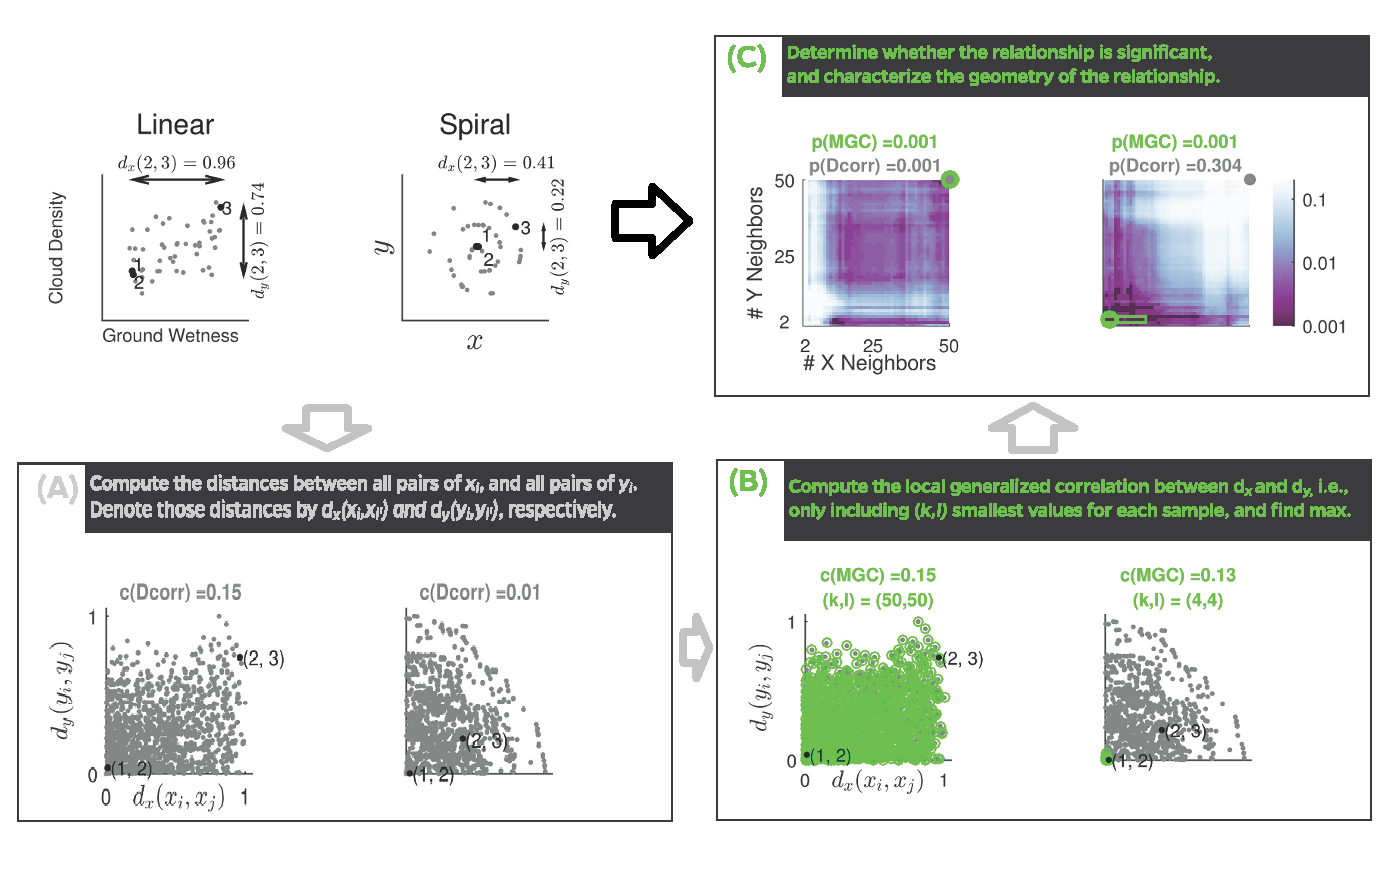
\includegraphics[width=1.0\textwidth]{Fig1All.png}
%\end{figure}
%\end{frame}

%\section{Theory}
%\begin{frame}{Population Form}
%\pause
%Assume that $(x_{i},y_{i}) \stackrel{i.i.d.}{\sim} F_{\mbx \mby}$ for all $i$, we can define the population local covariance by $dCov^{\rho_k,\rho_l}(\mbx,\mby)$ for $\rho_{k},\rho_{l} \in [0,1]$ via the characteristic functions of the underlying random variables, or Euclidean distances between pairs of i.i.d. random variables.

%\pause
%\medskip
%Similarly one can cast local variances / correlations / \Mgc~into the population form.

%\pause
%\medskip
%The population \Mgc~is directly connected to the sample version, and facilitates a number of desirable properties.
%See [\textit{Shen et al.(2017b)}]\cite{ShenEtAl2018} for more details.
%\end{frame}

%\begin{frame}{Population Form}
%\pause
%\begin{defi*}
%Let $\mb{I}(\cdot)$ be the indicator function, define two random variables
%\begin{align*}
%\mb{I}_{\mbx,\mbx'}^{\rho_{k}} &=\mb{I}(Prob\{B(\mbx,\|\mbx'-\mbx\|)\} \leq \rho_{k})  \\
%\mb{I}_{\mby',\mby}^{\rho_{l}} &=\mb{I}(Prob\{B(\mby',\|\mby-\mby'\|)\} \leq \rho_{l})
%\end{align*}
%with respect to the balls $B(\mbx,\|\mbx'-\mbx\|)$ and $B(\mby',\|\mby-\mby'\|)$ centered at $\mbx$ and $\mby'$ respectively.

%Suppose $(\mbx,\mby),(\mbx',\mby'),(\mbx'',\mby''),(\mbx''',\mby''')$ are i.i.d. as $F_{\mbx \mby}$, and define
%\begin{align*}
%d^{\rho_{k}}_{\mbx} &=(\| \mbx-\mbx' \| - \|\mbx-\mbx''\|) \mb{I}_{\mbx,\mbx'}^{\rho_{k}}, \\
%d^{\rho_{l}}_{\mby'} &=(\| \mby'-\mby \| - \|\mby'-\mby'''\|) \mb{I}_{\mby',\mby}^{\rho_{l}}.
%\end{align*}

%Then the population local covariance equals
%\begin{align}
%\label{eq:dcov2}
%dCov^{\rho_k, \rho_l}(\mbx,\mby) = E(d^{\rho_{k}}_{\mbx} d^{\rho_{l}}_{\mby'}) - E(d^{\rho_{k}}_{\mbx}) E(d^{\rho_{l}}_{\mby'}).
%\end{align}
%\end{defi*} 
%\end{frame}

%\begin{frame}{Properties of Population Local Correlation}
%\pause
%\begin{thm}
%\label{thm2}
%The population local correlation satisfies the following:
%\begin{description}
%\item [(a)] For any $(\rho_k,\rho_l) \in [0,1] \times [0,1]$, $dCorr^{\rho_{k},\rho_{l}}(\mbx,\mby)=dCorr^{\rho_{l},\rho_{k}}(\mby,\mbx) \in [-1,1]$.
%\item [(b)] If $\mbx$ is non-degenerate and $(\mbx, \mby)$ are dependent via a linear transformation (i.e., scaling, translation, rotation, reflection), then $dCorr^{\rho_{k},\rho_{l}}(\mbx,\mby)=1$ for all $\rho_k=\rho_l \in (0,1]$.
%\item [(c)] Under fixed marginals, $dCov^{\rho_{k},\rho_{l}}(\mbx,\mby)$ is a scalar multiple of $dCorr^{\rho_{k},\rho_{l}}(\mbx,\mby)$ regardless of the joint distribution, for any fixed $(\rho_k,\rho_l) \in [0,1] \times [0,1]$.
%\item [(c)] At $(\rho_k,\rho_l)=(1,1)$, $dCorr^{\rho_{k},\rho_{l}}(\mbx,\mby) = dCorr(\mbx,\mby)$.
%\item [(d)] For any $(\rho_k,\rho_l) \in [0,1] \times [0,1]$, $dCorr^{\rho_{k},\rho_{l}}(\mbx,\mby) = 0$ under the null (i.e., $\mbx$ is independent of $\mby$).
%\end{description}
%\end{thm}

%\pause
%\medskip
%(a-c) are also satisfied by the sample version $dCov^{kl}(X_{n},Y_{n})$, while (d) holds asymptotically for the sample version. These properties are also inherited by \Mgc~as a smoothed maximal local correlation.
%\end{frame}

%\begin{frame}{Convergence property}
%\pause
%We prove that the sample version converges to the population version as $n$ increases, and establish the convergence rate.

%\pause
%\medskip
%\begin{thm}
%\label{thm4}
%Suppose each column of $X_{n}$ and $Y_{n}$ are i.i.d. as $\mbx$ and $\mby$ respectively with finite second moments, sample local covariance satisfies
%\begin{align*}
%E(dCov^{kl}(X_{n},Y_{n})) &= dCov^{\rho_{k},\rho_{l}}(\mbx,\mby) +\mathcal{O}(1/n) \\
%Var(dCov^{kl}(X_{n},Y_{n})) &= \mathcal{O}(1/n)\\
%dCov^{kl}(X_{n},Y_{n}) &\stackrel{n \rightarrow \infty}{\rightarrow} dCov^{\rho_{k},\rho_{l}}(\mbx,\mby),
%\end{align*}
%where $\rho_{k}=\frac{k-1}{n-1}$ and $\rho_{l}=\frac{l-1}{n-1}$. In particular, the convergence is uniform for all sample local covariances, and also holds for the local correlations.
%\end{thm}
%\end{frame}

%\begin{frame}{Consistency of MGC}

%We can similarly define the population version of \Mgc, prove sample \Mgc~converges to the population \Mgc, and then testing consistency.\\

%\pause
%\medskip

%\begin{thm}
%\label{thm8}
%Suppose each column of $X_{n}$ and $Y_{n}$ are i.i.d. as $\mbx$ and $\mby$ of finite second moments, then $\GG^{*}(X_{n},Y_{n}) \geq 0$ asymptotically with equality if and only if independence. Therefore, at any type $1$ error level $\alpha>0$, \Mgc~is a valid test statistic that is consistent against all possible alternatives under the permutation test.
%\end{thm}
%\end{frame}

%\begin{frame}{Advantage of MGC over Dcorr}
%\pause
%Whenever there exist some local correlations that are larger than global distance correlation (1D non-monotone relationships), we prove that sample \Mgc~is larger than Dcorr as sample size increases.\\
%\pause
%\medskip
%\begin{thm}
%\label{thm7}
%Suppose each column of $X_{n}$ and $Y_{n}$ are i.i.d. as continuous $\mbx$ and $\mby$ respectively, and 
%\begin{align*}
%\max_{ (\rho_k,\rho_l) \in [0,1] \times [0,1]} \{dCorr^{\rho_{k},\rho_{l}}(\mbx,\mby)\} > Dcorr(\mbx, \mby).
%\end{align*}
%Then for $n$ sufficiently large, it holds that $\GG^{*}(X_{n}, Y_{n}) > Dcorr(X_{n}, Y_{n})$ for any threshold choice $\tau \rightarrow 0$.
%\end{thm}
%\pause
%\medskip
%Together with the smoothing step that mitigates the sample bias of \Mgc~under the null, the advantage on test statistic is translated to better finite-sample testing power of \Mgc~for nonlinear relationships. \\
%\end{frame}

%tba: add PIE and WIKI GF data
%\begin{frame}[allowframebreaks]
%\frametitle{References}
%\tiny
%\bibliographystyle{ieeetr}
%\bibliography{references}

%\end{frame}
\begin{frame}%[allowframebreaks]
\frametitle{References}
\small

1. \textcolor{UniOrange}{C. Shen}, C. E. Priebe, and J. T. Vogelstein, ``From distance correlation to the
multiscale graph correlation," Journal of the American Statistical Association, 2019.\\
\bigskip
2. J. T. Vogelstein, E. Bridgeford, Q. Wang, C. E. Priebe, M. Maggioni, and \textcolor{UniOrange}{C. Shen},
``Discovering and Deciphering Relationships Across Disparate Data Modalities," eLife, 2019.\\
\bigskip
3. Y. Lee, \textcolor{UniOrange}{C. Shen}, and J. T. Vogelstein, ``Network dependence testing via diffusion
maps and distance-based correlations," Biometrika, 2019.\\
\bigskip
4. S. Wang, \textcolor{UniOrange}{C. Shen}, A. Badea, C. E. Priebe, and J. T. Vogelstein, ``Signal
subgraph estimation via iterative vertex screening," under review.\\
\bigskip
5. \textcolor{UniOrange}{C. Shen} and J. T. Vogelstein, ``The Exact Equivalence of Distance and Kernel Methods for Hypothesis Testing," under review.\\
\if1\blind
{
\bigskip
5. \textcolor{UniOrange}{C. Shen} and J. T. Vogelstein, ``Characterizing dependency structure by the MGC image," \textit{in prep}.\\
\bigskip
6. \textcolor{UniOrange}{C. Shen}, Y. Lee, C. E. Priebe, and J. T. Vogelstein, ``K-sample testing via
multiscale graph correlation," \textit{in prep}.
}\fi
%\bibliographystyle{ieeetr}
%
\end{frame}

\addtocounter{framenumber}{-1} 
\begin{frame}<0> 
\bibliography{MGCbib}
\end{frame} 
%\bibliography{MGCbib}
%------------------------------------------------

%----------------------------------------------------------------------------------------

\end{document} 
